%  LaTeX support: latex@mdpi.com
%  For support, please attach all files needed for compiling as well as the log file, and specify your operating system, LaTeX version, and LaTeX editor.

%=================================================================
\documentclass[axioms,article,submit,pdftex,moreauthors]{Definitions/mdpi} 


% For posting an early version of this manuscript as a preprint, you may use "preprints" as the journal. Changing "submit" to "accept" before posting will remove line numbers.

%---------
% article
%---------
% The default type of manuscript is "article", but can be replaced by: 
% abstract, addendum, article, book, bookreview, briefreport, casereport, comment, commentary, communication, conferenceproceedings, correction, conferencereport, entry, expressionofconcern, extendedabstract, datadescriptor, editorial, essay, erratum, hypothesis, interestingimage, obituary, opinion, projectreport, reply, retraction, review, perspective, protocol, shortnote, studyprotocol, systematicreview, supfile, technicalnote, viewpoint, guidelines, registeredreport, tutorial
% supfile = supplementary materials

%----------
% submit
%----------
% The class option "submit" will be changed to "accept" by the Editorial Office when the paper is accepted. This will only make changes to the frontpage (e.g., the logo of the journal will get visible), the headings, and the copyright information. Also, line numbering will be removed. Journal info and pagination for accepted papers will also be assigned by the Editorial Office.

%------------------
% moreauthors
%------------------
% If there is only one author the class option oneauthor should be used. Otherwise use the class option moreauthors.

%---------
% pdftex
%---------
% The option pdftex is for use with pdfLaTeX. Remove "pdftex" for (1) compiling with LaTeX & dvi2pdf (if eps figures are used) or for (2) compiling with XeLaTeX.

%=================================================================
% MDPI internal commands - do not modify
\firstpage{1} 
\makeatletter 
\setcounter{page}{\@firstpage} 
\makeatother
\pubvolume{1}
\issuenum{1}
\articlenumber{0}
\pubyear{2024}
\copyrightyear{2024}
%\externaleditor{Academic Editor: Firstname Lastname}
\datereceived{ } 
\daterevised{ } % Comment out if no revised date
\dateaccepted{ } 
\datepublished{ } 
%\datecorrected{} % For corrected papers: "Corrected: XXX" date in the original paper.
%\dateretracted{} % For corrected papers: "Retracted: XXX" date in the original paper.
\hreflink{https://doi.org/} % If needed use \linebreak
%\doinum{}
%\pdfoutput=1 % Uncommented for upload to arXiv.org
%\CorrStatement{yes}  % For updates

\setlength{\headheight}{20.0pt} %% added from overleaf suggestion GP

%\newtheorem{definition}{Definition}
%=================================================================
% Add packages and commands here. The following packages are loaded in our class file: fontenc, inputenc, calc, indentfirst, fancyhdr, graphicx, epstopdf, lastpage, ifthen, float, amsmath, amssymb, lineno, setspace, enumitem, mathpazo, booktabs, titlesec, etoolbox, tabto, xcolor, colortbl, soul, multirow, microtype, tikz, totcount, changepage, attrib, upgreek, array, tabularx, pbox, ragged2e, tocloft, marginnote, marginfix, enotez, amsthm, natbib, hyperref, cleveref, scrextend, url, geometry, newfloat, caption, draftwatermark, seqsplit

\usepackage{accents}
\usepackage{amsmath,amssymb,amsthm}
\usepackage{graphicx}
\usepackage{mathtools}
\usepackage{soul}

%=================================================================
% Please use the following mathematics environments: Theorem, Lemma, Corollary, Proposition, Characterization, Property, Problem, Example, ExamplesandDefinitions, Hypothesis, Remark, Definition, Notation, Assumption
%% For proofs, please use the proof environment (the amsthm package is loaded by the MDPI class).
\theoremstyle{plain}
\newtheorem{theo}{Theorem}
% \theoremstyle{definition}
\newtheorem{mydef}{Definition}
\theoremstyle{remark}
\newtheorem{myexample}{Example}
%=================================================================
% Full title of the paper (Capitalized)
\Title{A Unified Approach to Aitchison's, Dually Affine, and Transport Geometries of the Probability Simplex}

% MDPI internal command: Title for citation in the left column
\TitleCitation{Title}

% Author Orchid ID: enter ID or remove command
\newcommand{\orcidauthorA}{0000-0000-0000-000X} % Add \orcidA{} behind the author's name
%\newcommand{\orcidauthorB}{0000-0000-0000-000X} % Add \orcidB{} behind the author's name

% Authors, for the paper (add full first names)
\Author{Giovanni Pistone $^{1,\ddagger}$\orcidA{0000-0003-2841-788X} and Muhammad Shoaib $^{2,\ddagger}$\orcidA{0009-0001-4064-0091}}

%\longauthorlist{yes}

% MDPI internal command: Authors, for metadata in PDF
\AuthorNames{Giovanni Pistone and Muhammad Shoaib}

% MDPI internal command: Authors, for citation in the left column
\AuthorCitation{Pistone G; Shoaib M}
% If this is a Chicago style journal: Lastname, Firstname, Firstname Lastname, and Firstname Lastname.

% Affiliations / Addresses (Add [1] after \address if there is only one affiliation.)
\address[1]{%
$^{1}$ \quad De Castro Statistics Initiative, Collegio Carlo Alberto; giovanni.pistone@carloalberto.org
\\ $^{2}$ \quad DIMA; muhammad.shoaib@dima.unige.it}

% Contact information of the corresponding author
\corres{Correspondence: muhammad.shoaib@dima.unige.it}

% Current address and/or shared authorship
%\firstnote{Current address: Affiliation.}  % Current address should not be the same as any items in the Affiliation section.
%\secondnote{These authors contributed equally to this work.}
% The commands \thirdnote{} till \eighthnote{} are available for further notes

%\simplesumm{} % Simple summary

%\conference{} % An extended version of a conference paper

% Abstract (Do not insert blank lines, i.e. \\) 
\abstract{A critical processing step of AI  algorithms is mapping the raw data to a landscape where the similarity of two data points is conveniently defined. Frequently, when the data points are compositions or probability functions, the similarity reduces to affine geometric concepts, where the basic notion is that of the straight line connecting two data points, defined as a zero acceleration line segment. This paper gives an axiomatic presentation of the probability simplex's most commonly used affine geometries. One result is a coherent presentation of gradient flow in Aichinson's Compositional Data, Amari's Information Geometry, Kantorivich distance, and Lagrangian optimization on the Probability Simplex.}

% Keywords
\keyword{Affine Geometry, Bayes Space, Information Geometry} 

% The fields PACS, MSC, and JEL may be left empty or commented out if not applicable
%\PACS{J0101}
%\MSC{}
%\JEL{}

%%% authors' macros
 
\newcommand{\CLR}{\operatorname{CLR}}
\newcommand{\clr}{\operatorname{clr}}
\newcommand{\Cov}{\operatorname{Cov}}
\newcommand{\Derivby}[1]{\frac{D}{d#1}}
\newcommand{\Entropy}{\mathcal H}
\newcommand{\Expat}[2]{\Exp_{#1}\left(#2\right)}
\newcommand{\Expectation}{\mathbb E}
\newcommand{\Exp}{\operatorname{Exp}}
\newcommand{\Grad}{\operatorname{grad}}
\newcommand{\KL}[2]{\operatorname{D}\left(#1\,\Vert#2\right)}
\newcommand{\acceleration}[1]{\accentset{**}{#1}}
\newcommand{\clrof}[2]{\CLR_{#1}\left(#2\right)}
\newcommand{\condexpat}[3]{\Expectation_{#1}\left(#2 \middle| #3\right)}
\newcommand{\contrastson}[1]{\operatorname{CO}\left(#1\right)}
\newcommand{\covat}[3]{\Cov_{#1}\left(#2,#3\right)}
\newcommand{\covof}[2]{\Cov\left(#1,#2\right)}
\newcommand{\densitieson}[1]{\mathcal P\left(#1\right)}
\newcommand{\derivby}[1]{\frac{d}{d#1}}
\newcommand{\entropyof}[1]{\Entropy\left(#1\right)}
\newcommand{\etransport}[2]{\prescript{\text{e}}{} {\mathbb U} _ {#1} ^ {#2}}
\newcommand{\euler}{\mathrm{e}}
\newcommand{\expbundleat}[1]{S\pdensitieson{#1}}
\newcommand{\fullbundleat}[1]{\prescript{1}{}S^1\pdensitieson{#1}}
\newcommand{\expectat}[2]{\Expectation_{#1}\left[#2\right]}
\newcommand{\expfibreat}[2]{S_{#1}\pdensitieson{#2}}
\newcommand{\mixfibreat}[2]{\prescript{*}{}{S}_{#1}\pdensitieson{#2}}
\newcommand{\htransport}[2]{\prescript{0}{} {\mathbb U} _ {#1} ^ {#2}}
\newcommand{\mtransport}[2]{\prescript{\text{m}}{} {\mathbb U} _ {#1} ^ {#2}}
\newcommand{\nonnegreals}{\mathbb{R}_{\ge 0}}
\newcommand{\pdensitieson}[1]{\mathcal P_{>}\left(#1\right)}
\newcommand{\posreals}{\mathbb{R}_{>0}}
\newcommand{\reals}{\mathbb{R}}
\newcommand{\scalarat}[3]{\left\langle#2,#3\right\rangle_{#1}}
\newcommand{\scalarof}[2]{\left\langle#1,#2\right\rangle}
\newcommand{\setof}[2]{\left\{#1 \, \middle| \, #2 \right\}}
\newcommand{\set}[1]{\left\{#1\right\}}
\newcommand{\transport}[2]{{\mathbb U} _ {#1} ^ {#2}}
\newcommand{\velocity}[1]{\accentset{\star}{#1}}
\newcommand{\mDerivby}[1]{\frac{\prescript{m}{}D}{d#1}}
\newcommand{\eDerivby}[1]{\frac{\prescript{m}{}D}{d#1}}

\begin{document}

%%%%%%%%%%%%%%%%%%%%%%%%%%%%%%%%%%%%%%%%%%
%\setcounter{section}{-1} %% Remove this when starting to work on the template.
%\section{Introduction}

%The template details the sections that can be used in a manuscript. Note that the order and names of article sections may differ from the requirements of the journal (e.g., the positioning of the Materials and Methods section). Please check the instructions on the journal's authors' page to verify the correct order and names. For any questions, please contact the editorial office of the journal or support@mdpi.com. For LaTeX-related questions please contact latex@mdpi.com.%\endnote{This is an endnote.} % To use endnotes, please un-comment \printendnotes below (before References). Only journal Laws uses footnotes.

\tableofcontents

\section{Introduction} \label{sec:intro}
This paper discusses the geometry of the set of all probabilities whose support is a given finite set. The \emph{sample space} $\Omega$ is the set of possible outcomes of the experiment of interest.
% We will see later how to extend the construction to infinite sample spaces.

\subsection{Probability Simplex} \label{sec:probability-simplex} 
On the finite sample space \(\Omega\), a probability is characterized by its \emph{probability function}  \(q \in \reals^{\Omega}\), that is, the mapping \(\Omega \to \posreals\) (the set of non-negative real numbers), where the sum of the probabilities over all outcomes equals 1. Hence, the set of all probability functions, the \emph{probability simplex}, is
     \begin{equation} \label{eq:probability-simplex}
          \densitieson \Omega = \setof{q \colon \Omega \to \nonnegreals} {\sum_{x \in \Omega} q(x) = 1} \ .
        \end{equation}
%The case $\Omega = \set{1,2,3}$ is illustrated in fig.~\ref{fig: probability simplex}
    
%\begin{figure}[t]
    %\centering
 %   \input Images/probability-simplex.tex
  %  \label{fig: probability simplex}
%\end{figure}

The probability simplex is closed under mixtures. Given two probability functions $p,q  \in \densitieson \Omega$, the line segment joining  $p$ and $q$, 
\begin{equation} \label{eq:mixture}
 [0,1] \ni t \mapsto p(t) = (1-t)p + t q  \ , 
\end{equation}
lies entirely within  $\densitieson \Omega$. 

\subsection{Compositions} \label{sec:compositions}
According to \cite{aitchison:1986} and \cite{pawlowsky-glahn|egozcue|tolosana-delgado:2015}, a \emph{composition} $f$ on the sample space $\Omega$ is a positive function on $\Omega$, $f \colon \Omega \to \nonnegreals$. Two compositions $f$, $g$ are equivalent if there exists a constant $k \in \posreals$ such that $g = kf$. Each composition $f$ is normalized to a probability function by
\begin{equation}
    \nonnegreals^\Omega \ni f \mapsto \frac f {\sum_{x \in \Omega} f(x)} \in \densitieson \Omega \ .
\end{equation}

Two compositions are equivalent if, and only if, the normalized compositions are equal so that the set of equivalent compositions is the same as the probability simplex. However, the notion of the composition suggests a geometric structure other than the mixture of Equation~\eqref{eq:mixture}. Given compositions $f$ and $g$, the product $h = fg$ is a composition, and the proportionality relation holds. If $f _1 = k_1f$ and $g_1 = k_2 g$, then $f_1g_1 = (k_1k_2) fg$. Similarly for the exponentiation $(\alpha,f) \mapsto f ^ \alpha$, $\alpha \in \reals$. 

These two operations provide a way of connecting two probability functions with the so-called \emph{exponential arc},
\begin{equation} \label{eq:exponential-arc}
 [0,1] \ni  t \mapsto \frac{p^{1-t} q^t}{\sum_{x \in \Omega} p(x)q(x)} \in \densitieson \Omega \ .
\end{equation}
The set of all compositions with the operations we have just described is sometimes called \emph{Bayes Space} \cite{egozcue|pawlowsky-glahn|tolosana-delgado|ortego|van-den-boogaart:2012} because the Bayes formula is possibly the most important example of a normalized product of compositions.

The mixture \eqref{eq:mixture} and the exponential arc \eqref{eq:exponential-arc} will be central objects in the geometric presentation of the probability simplex.

\subsection{Polytopes and Simplexes} \label{sec:polytopes}

We need to review some basic facts of convex analysis, see, e.g., \cite{barvinok:2002} and \cite{lay2007convex}. A set $S$ in a Euclidean space  $\mathbb{R}^n$ is \emph{convex} if for any two points  $p,q \in S$, the line segment joining  $p$ and $q$ of Equation~\eqref{eq:mixture} lies entirely within $S$. The \emph{convex hull} of a set $P \in \reals^n$ is the set of all convex combinations of points in  $P$,
\begin{equation*}
    \operatorname{conv}(P) = \setof{ \sum_{i=1}^{k} \lambda_i {p}_i}{k \ge 1, {p}_i \in P, \lambda_i \geq 0, \sum_{i=1}^{k} \lambda_i = 1} \ , 
\end{equation*}
where the non-negative real numbers $\lambda_i$ are the weights or coefficients of the convex combination, and  ${p}_i$  are points in $P$. % \cite{de2000computational}.
In particular, a \emph{polytope} is the convex hull of a finite set of points. A minimal set of such points is the set of vertexes. % \cite{ziegler2012lectures}. 
The probability simplex on $\Omega$ (also called standard simplex in other fields) is the polytope whose vertexes are the delta probability functions $\delta_a(x) = (x=a)$ for all $a\in \Omega$, that is,
\begin{equation}
\delta_a(x) = \begin{cases} 
1 & \text{if } x = a, \\
0 & \text{otherwise}.
\end{cases}
\end{equation}
Each \(\delta_a\) represents a probability where the entire probability mass is concentrated at \(a\).

An \emph{affine combination} of the vectors $p_1,\dots,p_k \in \reals^\Omega$ is a vectors of the form $\sum_{j=1}^k t_j p_j$, with $\sum_{j=1}^k t_j = 1$. The given vectors are \emph{affinely independent} if no affine combination is zero. A \emph{simplex} is a polytope generated by \emph{affinely independent} points $a_1,\dots,a_n$. All simplexes with the same number of vertices can be transformed into one another by a suitable affine function. Thus, any \(n\)-vertex simplex in any \(n\)-dimensional space is essentially the same shape, differing only by scaling, rotation, and translation.
%This observation is relevant in the graphical representation of compositional data, as illustrated in fig.~\ref{fig: probability simplex}.

The probability simplex is a closed set in his ambient Euclidean space. The topological border is a union of simplexes of smaller dimensions, each one corresponding to a reduced support of the probability functions. In statistical modeling, one usually assumes that the support of each probability function in the model of interest is the same. For this reason, we will mainly consider the open probability simplex $\pdensitieson \Omega$, which is the set of strictly positive probability functions.

%Non parametric IG \cite{pistone|sempi:95}, Affine IG \cite{chirco|pistone:2022}.

\subsection{Overview}

This piece of research presents in a coordinated and principled way some basic topics in the geometrical calculus of the probability simplex. The specific topics are Aitchison's theory of compositional data and Bayes spaces, Amari's dually affine information geometry, and Transport theory in product sample spaces. We define a differential geometric structure with an explicitly defined expression of the tangent bundle and discuss the relevant calculus operations, especially the notions of natural gradient and of gradient flow.

Section~\ref{PS} is devoted to the definition of \emph{affine space} as a set $M$ endowed with a \emph{displacement} function that maps every couple of points to a vector in such a way the rule of addition of vectors holds. An affine space is a differentiable manifold where the displacement function with the first point fixed provides a chart from $\mathcal{M}$ to a vector space. The Aitchison geometry of compositional data is an instance of such a geometry.

Section~\ref{sec:statistical bundle} presents a generalization of the notion of affine space to a more complex object which allows us to set Information Geometry within this geometric framework. In affine spaces, the tangent space is the same at each point. However, the classical Fisher's methodology, together with Amari's methodology, suggests taking the Fisher's score as a definition of the tangent vector. As a consequence, it is convenient to assume that the primary expression of the tangent bundle is the set of weighted contrasts. This natural setting requires an extra structure, that is, an identification between tangent spaces, called a \emph{parallel transport}. This section contains the main computational results, particularly the notions of natural gradient, duality of transports, and gradient flow.

Section~\ref{sec:product-sample-space} presents the analysis of the affine statistical bundle when the sample space is of product type. In this case, we introduce the notions of ANOVA decomposition and optimal transport plan.

Section~\ref{sec:mechanics} deals with the second-order geometric analysis of the probability simplex, that is, the first-order geometric analysis of the statistical bundle. Computations inspired by methods from mechanics, such as the optimization of Lagrangian functions, Newton's method of optimization, and Hamiltonian dynamics, are not used much in statistics. The statistical bundle provides a methodology that is formally consistent and manageable.


\section{Affine Geometry of the Probability Simplex}
\label{PS}
The geometries we are going to discuss are supported on the probability simplex $\densitieson \Omega$ or {on}  the open probability simplex $\pdensitieson \Omega$ of a finite sample space $\Omega$. The latter open convex set is the interior of the former full probability simplex \eqref{eq:probability-simplex}. The term "geometry" is ambiguous and should be qualified by stating which type of geometry we are talking about. Actually, the field of statistics uses many types of geometries, such as linear, affine, metric, geodesic, Riemannian, and differential geometries. We discuss here about affine geometry, to be precisely defined below. Our general references are the monographs \cite{amari|nagaoka:2000}, \cite{amari:2016}, and \cite[Ch.~I-II]{nomizu|sasaki:94}. The tutorials \cite{pistone:2020-NPCS} and \cite{chirco|malago|pistone:2022} present similar material as the present one but in a more restricted scope. 

Affine geometry is a special instance of differential geometry. The former inherits the language of the latter: chart, atlas, expression, tangent space, bundle \dots. We refer to the non-parametric version of differential geometry as presented in \cite{bourbaki:71variete} and \cite{lang:1995}. Below, we list the basic concepts.

Given a set \( M \) and a real vector space \( V \), a \emph{chart} is a one-to-one mapping $s: U \to V$ where \( U \subset M \) and \( s(U) \) is open in \( V \). Two charts \( s_1 \colon U_1 \to V_1 \) and \( s_2 \colon U_2 \to V_2 \)
are
\( C^k \)-compatible if the change-of-chart mapping
\begin{equation*} 
s_2 \circ s_1^{-1}: s_1(U_1 \cap U_2) \to s_2(U_1 \cap U_2)
\end{equation*} 
is either empty or a \( C^k \)-diffeomorphism of open sets. (As usual $\circ$ stands for composition of functions.) A family of two by two \( C^k \)-compatible charts is a \( C^k \)-\emph{atlas}. 
Two atlases are compatible if their union is an atlas. A maximal $C^k$-atlas ia a $C^k$-\emph{manifold}.

A \emph{curve} is a map from a real interval to the manifold. We assume, unless otherwise stated, the interval to an open neighborhood of 0.
Given a curve $\gamma \colon t \mapsto \gamma(t) \in M$ and a chart $s$ in the atlas, the curve $s \circ \gamma \colon t \mapsto s(\gamma(t)) \in V$ is the \emph{expression} of the curve in the chart $s$. If one expression (hence all) is differentiable, then $t \mapsto \derivby t \, s \circ \gamma(t) \in V$ is the expression of the velocity at $t$ of the curve $\gamma$ in the chart $s$. The vector space of all possible expressions of velocities for curves passing through a given $p \in M$ is the expression of the \emph{tangent space} at $p$.  

\subsection{Affine Space}
The open probability simplex and the probability simplex $\pdensitieson\Omega$ are, respectively, an open convex subset and a closed convex subset of the generated hyperplane,
\begin{equation} \label{eq:hyperplane}
    A(\Omega) = \setof{{v} \in \reals^\Omega}{\sum_{x \in \Omega} v(x) =1} \ ,
\end{equation}
{where }$A(\Omega)$ consists of all vectors in the vector space $\reals^\Omega$ whose components sum to 1. Probability functions are non-negative and sum to 1. As $A(\Omega)$ is an Euclidean space, the open probability simplex inherits {the Euclidean} geometry. In some contexts, it is useful to relax the non-negativity constraint and allow the "probabilities" to take on negative values while maintaining the sum-to-one condition. By allowing $v(x)$ to be negative, we extend our consideration from the standard probability simplex to a larger space. 

\begin{myexample}
Consider a simple 3-dimensional probability space with outcomes \( \Omega = \{1, 2, 3\} \). A probability vector \( v \in \mathbb{R}^3 \) in this space might look like \( v = (v_1, v_2, v_3) \) where \( v_1 + v_2 + v_3 = 1 \).  For standard probabilities, we require \( v_1, v_2, v_3 \geq 0 \). However, if we relax this constraint, \( v_1, v_2, v_3 \) can assume negative values as long as they sum to 1.
In the plot of fig.~\ref{fig:Affine_score}, the blue triangle represents the standard probability simplex where \( v_1, v_2, v_3 \geq 0 \). The red points represent example vectors in the generalized affine space, including one where \( v_3 \) is negative and another where \( v_1 \) exceeds 1.
\begin{figure}[t]
    \centering
    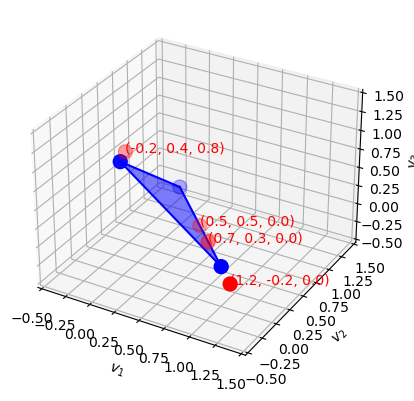
\includegraphics[scale = 0.5]{Images/affine_score.png}
    \caption{The blue triangle represents the probability simplex. Red points represent vectors in the generalized affine space, including points with negative values or values exceeding 1}
    \label{fig:Affine_score}
\end{figure}
\end{myexample}

\begin{myexample} \label{ex:Brier}
A \emph{score function} \( S \) can be defined on the space of these generalized probability vectors. For a given vector \( v \) and an outcome \( x \), the score \( S(v, x) \) quantifies how well the vector \( v \) predicts the outcome \( x \). A common example of a score function is the Brier score \cite{brier:1950VERIFICATIONOF}, defined as:
\begin{equation*} 
S(v, x) = \sum_{y \in \Omega} (v(y) - \delta_x(y))^2
\end{equation*} 
where \(\delta_x\) is the indicator function of $x$, that is, 1 if \( y = x \) and 0 otherwise. %The Brier score can be adapted to handle negative values in \( v \) by ensuring the squared differences are appropriately interpreted.
\end{myexample}

The following definition, due to \cite{weyl:1952}, extends the notion of geometry on a hyperplane to a more general situation.

\begin{mydef}[Weyl's affine space]
Given a set \( M \) and a real finite-dimensional vector space \( V \), an affine space \( (M, V, \overrightarrow{\cdot \cdot}) \) consists of a \emph{displacement mapping}
% \cite{amari2000methods}
\begin{equation*}
M \times M \ni (p, q) \mapsto \overrightarrow{pq} \in V \ ,
\end{equation*}
such that the following two assumptions hold.
\begin{enumerate}
    \item\label{item:one-to-one} For each point \( p \in M \), the partial mapping \( s_p : M \ni q \mapsto s_p(q) = \overrightarrow{pq} \) is injective (one-to-one) with open image $s_p(M)$. 
    \item \label{item:Chasles} Given points $p$, $q$, and $r$, the displacement vectors satisfy the parallelogram law,
   \begin{equation*}
   \overrightarrow{pq} + \overrightarrow{qr} = \overrightarrow{pr} \ .
   \end{equation*}
   \end{enumerate}
\end{mydef}

Property \ref{item:one-to-one} ensures that for a fixed point \( p \), the mapping from points in \( M \) to the vector space \( V \) via the displacement vector \( \overrightarrow{pq} \) does not map different points to the same vector. In the language of differential geometry, the mapping $s_p$ is a \emph{chart}, and $v = s_p(q)$ is the coordinate of $q$ in the $p$-chart. As $s_p(p) = 0$, we will say that $p$ is the \emph{origin} of the chart. The inverse chart, also called a \emph{patch}, is $s^{-1}_p \colon s_p(M) \to M$.

Property~\ref{item:Chasles} means that the vector displacement from \( p \) to \( r \) is the same as the sum of the vector displacement from \( p \) to \( q \) and from \( q \) to \( r \), see fig.~\ref{fig:aff_1}. This property ensures that adding displacements is consistent with the geometric intuition of moving along a path from one point to another via an intermediate point. In terms of the charts, 
\begin{equation} \label{eq:Chasles}
   s_p(q) + s_q(r) = s_p(r) \ .
   \end{equation}
      \begin{figure}[t]
    \centering
   \tikzset{every picture/.style={line width=0.75pt}} %set default line width to 0.75pt        
\begin{tikzpicture}[x=0.75pt,y=0.75pt,yscale=-1,xscale=1]
%uncomment if require: \path (0,300); %set diagram left start at 0, and has height of 300

%Shape: Rectangle [id:dp386585098716997] 
\draw   (362,89.5) -- (511,89.5) -- (511,170.5) -- (362,170.5) -- cycle ;
%Shape: Triangle [id:dp10995406038896904] 
\draw   (233,91.5) -- (346,169) -- (200,169) -- cycle ;
%Curve Lines [id:da0046823044336183894] 
\draw [color={rgb, 255:red, 74; green, 144; blue, 226 }  ,draw opacity=1 ]   (241,111.5) .. controls (246,125.5) and (277,165.5) .. (311,157.5) ;
\draw [shift={(311,157.5)}, rotate = 346.76] [color={rgb, 255:red, 74; green, 144; blue, 226 }  ,draw opacity=1 ][fill={rgb, 255:red, 74; green, 144; blue, 226 }  ,fill opacity=1 ][line width=0.75]      (0, 0) circle [x radius= 1.34, y radius= 1.34]   ;
\draw [shift={(241,111.5)}, rotate = 70.35] [color={rgb, 255:red, 74; green, 144; blue, 226 }  ,draw opacity=1 ][fill={rgb, 255:red, 74; green, 144; blue, 226 }  ,fill opacity=1 ][line width=0.75]      (0, 0) circle [x radius= 1.34, y radius= 1.34]   ;
%Straight Lines [id:da5831209167526987] 
\draw [color={rgb, 255:red, 189; green, 16; blue, 224 }  ,draw opacity=1 ]   (383,157.5) -- (444.02,148.78) ;
\draw [shift={(446,148.5)}, rotate = 171.87] [color={rgb, 255:red, 189; green, 16; blue, 224 }  ,draw opacity=1 ][line width=0.75]    (4.37,-1.32) .. controls (2.78,-0.56) and (1.32,-0.12) .. (0,0) .. controls (1.32,0.12) and (2.78,0.56) .. (4.37,1.32)   ;
%Straight Lines [id:da22052958952646162] 
\draw [color={rgb, 255:red, 189; green, 16; blue, 224 }  ,draw opacity=1 ]   (383,157.5) -- (414.93,107.19) ;
\draw [shift={(416,105.5)}, rotate = 122.4] [color={rgb, 255:red, 189; green, 16; blue, 224 }  ,draw opacity=1 ][line width=0.75]    (4.37,-1.32) .. controls (2.78,-0.56) and (1.32,-0.12) .. (0,0) .. controls (1.32,0.12) and (2.78,0.56) .. (4.37,1.32)   ;
%Straight Lines [id:da5541393906182921] 
\draw [color={rgb, 255:red, 189; green, 16; blue, 224 }  ,draw opacity=1 ]   (383,157.5) -- (472.31,101.56) ;
\draw [shift={(474,100.5)}, rotate = 147.94] [color={rgb, 255:red, 189; green, 16; blue, 224 }  ,draw opacity=1 ][line width=0.75]    (4.37,-1.32) .. controls (2.78,-0.56) and (1.32,-0.12) .. (0,0) .. controls (1.32,0.12) and (2.78,0.56) .. (4.37,1.32)   ;
\draw [shift={(383,157.5)}, rotate = 327.94] [color={rgb, 255:red, 189; green, 16; blue, 224 }  ,draw opacity=1 ][fill={rgb, 255:red, 189; green, 16; blue, 224 }  ,fill opacity=1 ][line width=0.75]      (0, 0) circle [x radius= 1.34, y radius= 1.34]   ;
%Straight Lines [id:da7616436025465434] 
\draw  [dash pattern={on 0.84pt off 2.51pt}]  (416,105.5) -- (474,100.5) ;
%Straight Lines [id:da8239235647250038] 
\draw  [dash pattern={on 0.84pt off 2.51pt}]  (446,148.5) -- (474,100.5) ;
%Curve Lines [id:da8012286103412225] 
\draw    (217,154.5) .. controls (222,129.5) and (233,122.5) .. (241,111.5) ;
\draw [shift={(241,111.5)}, rotate = 306.03] [color={rgb, 255:red, 0; green, 0; blue, 0 }  ][fill={rgb, 255:red, 0; green, 0; blue, 0 }  ][line width=0.75]      (0, 0) circle [x radius= 1.34, y radius= 1.34]   ;
\draw [shift={(217,154.5)}, rotate = 281.31] [color={rgb, 255:red, 0; green, 0; blue, 0 }  ][fill={rgb, 255:red, 0; green, 0; blue, 0 }  ][line width=0.75]      (0, 0) circle [x radius= 1.34, y radius= 1.34]   ;

% Text Node
\draw (253,173.4) node [anchor=north west][inner sep=0.75pt]    {$\mathcal{M}$};
% Text Node
\draw (432,175.4) node [anchor=north west][inner sep=0.75pt]    {$V$};
% Text Node
\draw (220,151.4) node [anchor=north west][inner sep=0.75pt]  [font=\scriptsize]  {$p$};
% Text Node
\draw (232,99.9) node [anchor=north west][inner sep=0.75pt]  [font=\scriptsize]  {$q$};
% Text Node
\draw (297,143.4) node [anchor=north west][inner sep=0.75pt]  [font=\scriptsize]  {$r$};
% Text Node
\draw (386.5,120.56) node [anchor=north west][inner sep=0.75pt]  [font=\scriptsize,rotate=-307.44]  {$\overrightarrow{pq}$};
% Text Node
\draw (415.27,119.74) node [anchor=north west][inner sep=0.75pt]  [font=\scriptsize,rotate=-327.17]  {$\overrightarrow{pr}$};
% Text Node
\draw (426,136.4) node [anchor=north west][inner sep=0.75pt]  [font=\scriptsize]  {$\overrightarrow{qr}$};
% Text Node
\draw (368.51,160.01) node [anchor=north west][inner sep=0.75pt]  [font=\scriptsize,color={rgb, 255:red, 0; green, 0; blue, 0 }  ,opacity=1 ,rotate=-330.07]  {$O$};
\end{tikzpicture}
\caption{Parallelogram law in an affine space}
    \label{fig:aff_1}
\end{figure}
   
In particular, we have $s_p(p) = \overrightarrow{pp} = 0$, hence $s_p$ is the chart centred at $p$. Also, $s_p(q) + s_q(p) = 0$. The change-of-chart transformation from origin $p$ to origin $q$ follows from Equation~\eqref{eq:Chasles}
\begin{equation} \label{eq:change-of-charts}
  s_q \circ s^{-1}_p (v) =s_q(s^{-1}_p (v)) = s_q(p) + s_p(s^{-1}_p (v)) = s_q(p) + v \ .
\end{equation}
The change-of-chart from origin $p$ to origin $q$ is the translation by $s_q(p) = - s_p(q)$.

\subsection{Affine Manifold}
In the affine space \( (M, V, \overrightarrow{\cdot \cdot}) \), the displacement \( (p,q) \mapsto \overrightarrow{pq} \) defines a system of charts $s_p \colon M \ni q \mapsto \overrightarrow{pq}$ as $p$ varies in $\mathcal{M}$. 
Each $s_p$ is one-to-one, and the change-of-charts~\eqref{eq:change-of-charts} are translations, hence highly smooth. The \emph{affine manifold}  is defined by the atlas of charts \( s_p : M \to V \), \( p \in M \). The affine manifold differs from the $C^k$-manifold it generates because the former is not maximal as the latter. Any vector basis of \(V\) provides a version of the affine space where the vector space is a real vector space of parameters, producing a faithful parametrization of \(M\).

Consider a curve \( t \mapsto \rho(t) \in M \) in the affine manifold. For any reference point \( p \in M \), the curve \( t \mapsto s_p(\rho(t)) \) is the $s_p$-expression of the curve. The derivative $
\frac{d}{dt} s_p(\rho(t))$ does not depend on the choice of the point \( p \):
\begin{equation*} 
\frac{d}{dt} s_p(\rho(t)) = \frac{d}{dt} \left( s_p(q) + s_q(\rho(t)) \right) = \frac{d}{dt} s_q(\rho(t))
\end{equation*} 
Thus, the derivative \( \displaystyle \frac{d}{dt} s_p(\rho(t)) \) is independent of the choice of \( p \) and is called the \emph{affine velocity of the curve} and is denoted by
\begin{equation*}
\Derivby t \rho(t) \quad \text{or} \quad \velocity q(t) \ .
\end{equation*}

The vector space of all velocities evaluated at $t = 0$ of all curves $t \mapsto \rho(t) \in M$ such that $\rho(0) = p$, is the \emph{tangent space} at $p$ of the affine manifold, namely
\begin{equation}
    T_p = \setof{\velocity q(0)}{t \mapsto q(t) \in M, q(0) = p}
\end{equation}
Conversely, given any $v \in V$, the curve $t \mapsto s_p^{-1}(tv)$ has affine velocity $v$, so that $T_p M = V$.

\begin{myexample}
\label{ex:contrasts}
Let us discuss a basic elementary example that is relevant in the statistical literature of design of experiment and regression modelling.
If we take as base set \(M\) the hyperplane $A(\Omega)$ of Equation~\eqref{eq:hyperplane} and as vector space the vector space parallel to the probability simplex, that is, the space of \emph{contrasts},
\begin{equation} \label{eq:contrasts}
\contrastson\Omega = \setof{ v \in \reals^\Omega}{\sum_{x \in \Omega} v(x) = 0} \ ,
\end{equation}
the displacement is \(\overrightarrow{pq} = q - p \in V\). In fact, \(\sum_{x} (q(x) - p(x)) = 1 - 1 = 0\). and the mapping \(s_p(q) = q - p\) is one-to-one and onto. The parallelogram law is \((q - p) + (r - q) = (r - p)\). The tangent space is defined in Equation~\eqref{eq:contrasts}. In the case
with \(\Omega = \set{1, 2, 3}\), a vector basis of $\contrastson\Omega$ is
\begin{equation*} 
v_1 = (1, -1, 0), \quad v_2 = (1, 0, -1) \ ,
\end{equation*} 
so that
\begin{equation*} 
(p, q) \mapsto s_p(q) = -(q(2) - p(2))
\begin{pmatrix}
1 \\
-1 \\
0
\end{pmatrix}
- (q(3) - p(3))
\begin{pmatrix}
1 \\
0 \\
-1
\end{pmatrix} \ .
\end{equation*} 
The chart at $p$ in parametric coordinates is
\begin{equation*} q \mapsto 
\begin{pmatrix}-(q(2) - p(2)) \\ -(q(3) - p(3))\end{pmatrix} \in 
\reals^2 \ .
\end{equation*} 
Often, interpretability of regression models depends on the suitable choice of vector space bases of $\contrastson\Omega$ and charts.
\end{myexample}

Interestingly, many types of affine manifolds on the open probability simplex are of statistical interest. They all use the space of contrasts \eqref{eq:contrasts} as vector space. Various vector bases of $\contrastson\Omega$ are commonly used in applications. One option is to choose a component $a \in \Omega$ and use the \emph{reduced basis} $(\delta_x)_{x \neq a}$. With this basis, the components of the projection of $v \in \contrastson\Omega$ are $(v(x) - v(a))_{x \neq a}$. A second option is the \emph{preferred point basis}. Fix $a \in \Omega$. If $v$ is a contrast, it holds $v(a) = - \sum_{x \neq a} v(x)$, hence $v = \sum_{x \neq a} v(x) (\delta_x - \delta_a)$ and $(\delta_x - \delta_a)_{x \neq a}$ is a basis. 

The space of contrasts is an Euclidean space, for example, with the restriction of the inner product in $\reals^\Omega$. Other inner products are used.  While not part of the affine geometry, these metrics, applied to the vector space of contrasts, provide various useful instances of metric on the affine space, see ex.~\ref{ex:Brier}. It is important to realize that the choice of an affine displacement and the choice of an inner product are independent modeling choices.

\begin{myexample}[Open Probability Simplex] \label{ex:A}
The construction in Example~\ref{ex:contrasts} is not feasible on the probability simplex because the image of the restricted mapping
\begin{equation*}
    \densitieson\Omega \colon q \mapsto q - p \in \contrastson\Omega
\end{equation*}
is closed. We can use the same construction as before if we restrict to the open probability simplex,
\begin{equation}
    \pdensitieson\Omega \colon q \mapsto q - p \in \contrastson\Omega
\end{equation} 
\end{myexample}

\subsubsection{Aitchison's Centred Log-Ratio \cite{aitchison:1986}}
\label{sec:aitchison-clr}
In this section, a key notion for statistical usage of Aitchison's geometry, namely the centered log ratio ($\clr$), is interpreted as a displacement. This allows the interpretation of the moments of a random variable of the cumulant function in this framework. 

%\begin{myexample}[] \label{ex:B} 
If $f$ and $f_1 = k_1 f$ are equivalent positive compositions, then $\log f_1 = \log f + \log k_1$. The logarithms of equivalent compositions differ by an additive constant. This remark suggests using a logarithmic scale by considering the set of positive probability functions $\pdensitieson\Omega$, the vector space of contrasts $\contrastson\Omega$, $n = \#\Omega$, and \emph{centred log-ratio} displacement
\begin{equation}\label{eq:CLR}
\CLR \colon \pdensitieson\Omega \times \pdensitieson\Omega \ni (p,q) \mapsto \log \frac q p - \sum_{x \in \Omega} \frac 1{n} \log \frac{q(x)}{p(x)} \ .
\end{equation}
If $f$ is a composition and $\phi$ is a random variable on $\Omega$, we define the $\Expectation$-notation to include normalization, 
\begin{equation}
    \expectat f \phi = \sum_{x \in \Omega} \frac{f(x)}{\sum_x f(x)} \, \phi(x) \ .
\end{equation}

Let us check that all conditions for an affine manifold hold. The partial mapping at p is a chart with
\begin{gather}
 s_p \colon \pdensitieson\Omega \ni q \mapsto \clrof p q  = \log \frac q p - \expectat 1 {\log \frac q p} \in \contrastson\Omega \ , \label{eq:CLR+1} \\
 s^{-1}_p \colon \contrastson\Omega \ni v \mapsto \euler^{v - \Psi_p(v)} \cdot p \quad \ , \quad \Psi_p(v) = \expectat 1 {\log \frac p q} = \log \expectat p {\euler^v} \label{eq:CLR-1} \ .
    \end{gather}

The axioms for affine geometry are satisfied, as the equality $s_p(q) + s_q(r) = s_p(r)$ is easily checked,
\begin{multline*}
    \clrof p q + \clrof q r = \log \frac q p - \expectat 1 {\log \frac q p } + \log \frac r q  - \expectat 1 {\log \frac rq}  \\
    = \log \frac r p - \expectat 1 {\log \frac r p} = \clrof p r \ .\end{multline*}
% \end{myexample}

%\begin{myexample}[\textcolor{red}{Curve's kinematics in Aitchison geometry}]
The patch mapping is a non-parametric exponential model \cite{brown:86} or \cite[\S~5.5]{efron|hastie:2016} where the sufficient statistics $v$ is a contrast. The convex mapping $\Psi_p$ is sometimes called a cumulant function. The first and second derivatives of $\Psi_p$ in the direction $h$ and the directions $h$ and $k$, respectively, are (as computed in the references above),
\begin{equation} \label{eq:cumulant-derivs}
  d \Psi_p(v)[h] =  \expectat q h \ , \quad d^2 \Psi_p(v)[h,k] = \covat q h k \ .
\end{equation}

    The velocity of the curve $t \mapsto q(t)$ is
    \begin{equation*}
        \derivby t \clrof p {q(t)} = \derivby t \log q(t) - \expectat 1 {\derivby t \log q(t)} = \frac{\dot q(t)}{q(t)} - \expectat 1 {\frac{\dot q(t)}{q(t)}} \ .
    \end{equation*}
    where $\dot q(t)$ is the derivative computed in $A(\Omega)$. The random variable $\dot q(t) / q(t)$ is called \emph{Fisher's score} \cite{efron|hastie:2016} and has the remarkable property
    \begin{equation*}
        \expectat {q(t)} {\frac{\dot q(t)}{q(t)}} = \sum_{x \in \Omega} \dot q(x;t) = 0 \ .
    \end{equation*}

    In the reduced basis, with $\Omega = \set{1,\dots,n}$, each $j \neq n$ component of the $\CLR$ displacement becomes
    \begin{multline*}
  \clrof p q(j) = \left(\log \frac{q(j)}{p(j)}  - \expectat 1 {\log \frac{q}{p}}\right) - \left(\log \frac{q(j)}{p(j)}  - \expectat 1 {\log \frac{q}{p}}\right)  \\ 
 = \log \frac{q(j)}{p(j)} -\log \frac{q(n)}{p(n)}  = \log \frac{p(n)q(j)}{p(j)q(n)} \ .
  \end{multline*}
  See \cite{pawlowsky-glahn|egozcue|tolosana-delgado:2015} for a detailed treatment.
% \end{myexample}

Within Aitchison's paradigm, we presented the idea of the centred log-ratio (CLR) transformation \eqref{eq:CLR}. Determining displacement mappings between probability distributions on the simplex depends critically on this transformation. By mapping compositions into a Euclidean space, the CLR makes easier the comparison and analysis of probability distributions in a way that makes sense with respect to the inherent geometry of the simplex (refers to the unique geometric properties of the probability simplex—a space that consists of probability distributions where all components are positive and sum to one.). Aitchison geometry's mathematical foundations are explored in more detail in  Section~\ref{AG} with special attention on how it relates to information geometry (IG). We discuss how Aitchison geometry may be considered a specific example of IG, simplifying the displacement mappings with a fixed reference chart and deriving important conclusions, including the parallelogram law that guarantees these mappings to be consistent over a wide range of distributions. Further explanation and detailed connections with the centred log-ratio transformation are provided in Section ~\ref{AG} below.

\subsection{Tangent Bundle} 

The motivation for defining a manifold structure $\mathcal M$ through an atlas $\mathcal A$ is the availability of a coherent setup for performing calculus operations. A typical problem of our interest is minimizing a smooth scalar field $G \colon \mathcal M \to \reals$ via a gradient flow algorithm. To this end, we must consider points on the manifold and derivatives, which live in a vector space attached to each point.

The \emph{tangent bundle} $T \mathcal M$ is defined as a set of pairs 
\begin{equation*} 
T \mathcal M = \setof{(q,v)}{q \in \mathcal M, v \in T_q \mathcal M} \ ,
\end{equation*} 
where $T_q \mathcal M$ is the tangent space at $q$, that is, the vector space of all possible velocities of curves through $q$. The situation is straightforward in all the examples of affine manifold we have seen up to now, as the tangent space identifies with the space of contrasts $\contrastson\Omega$.

\begin{myexample}[Exponential arc] Let $t \mapsto p(t)$ be the exponential arc in Equation~\eqref{eq:exponential-arc} connecting the points $q$ and $r \in \pdensitieson\Omega$. In the CLR affine manifold, we represent the two equivalent probability densities  with the CLR patch centred at $p$ as in Equation~\eqref{eq:CLR-1},
\begin{equation*}
    q = \euler^{v - \Psi_p(v)} \cdot p \ , \quad r = \euler^{w - \Psi_p(w)} \cdot p \ , \quad 
   with \,\, v,w \in \contrastson\Omega \ ,
\end{equation*}
hence the arc $t \mapsto p(t)$ is expressed in terms of a mixture of two random variables $v$ and $w$ and the convex mapping $\Psi_p$, that is, two canonical statistics and the cumulant function,
\begin{equation*}
    p(t) = \euler^{(1-t)v + t w - \Psi_p((1-t) v + t w)} \cdot p \quad \text{and} \quad \clrof p {p(t)} = (1-t) v + t w \ .
\end{equation*}

The affine velocity is constant,
\begin{equation*}\velocity q(t) = \derivby t \clrof p {p(t)} = \derivby t ((1-t)v - tw) = w -v \ .
\end{equation*}
The exponential arc is the line segment with constant velocity connecting $q$ and $r$ in the CLR affine geometry. The set of all possible velocities at a given point is an expression of the tangent space.
\end{myexample}

\begin{myexample}[Gradient of the KL-divergence] For any $p \in \pdensitieson\Omega$, the Kullback–Leibler divergence, in short KL-divergence (see \cite{cover|thomas:2006} or \cite[\S~3.3-4]{amari:2016}), of $q$ and $p$ is the scalar field
\begin{equation*}
    \pdensitieson \Omega \ni q \mapsto \KL p q = \expectat p {\log \frac p q} \in \reals \ .
\end{equation*}

The patch at $p$ for the CLR displacement is Equation~\eqref{eq:CLR-1} hence the expression at $p$ of the KL-divergence is 
\begin{equation*}
  G \colon  v \mapsto \KL p {\euler^{v - \Psi_p(v)} \cdot p} = \expectat p {-v + \Psi_p(v)} = \Psi_p(v) - \expectat p v \ .
\end{equation*}
The expression is defined on the vector space $\contrastson\Omega$ and hence, we can  compute the ordinary derivative in the direction $h \in \contrastson\Omega$ using Equation~(\ref{eq:cumulant-derivs}) and $q = \euler^{v - \Psi_p(v)} \cdot p$,
\begin{multline*}
    dG(v)[h] = \left. \derivby t G(v + th) \right|_{t=0} = \left. \derivby t \Psi_p(v + th) \right|_{t=0} - \expectat p h \\ 
    = d\Psi_p(v)[h] - \expectat p h = \expectat q h - \expectat p h 
 =  \expectat p {(\euler^{v - \Psi_p(v)} - 1))h} \\ 
 = \expectat 1 {np(\euler^{v - \Psi_p(v)} - 1) h} \ . \end{multline*}

As  $np(\euler^{v - \Psi_1(v)} - 1) \in \contrastson\Omega$, if we define the inner product of $\contrastson\Omega$ to be $(v,w) \mapsto \scalarof v w = \expectat 1 {vw}$, then $np(\euler^{v - \Psi_1(v)} - 1)$ is the \emph{gradient} of $G$,
\begin{equation*}
    dG(v)[h] = \scalarof{pn(\euler^{v-\Psi_p(v)}}{h} \ .
\end{equation*}

The gradient is also defined on the affine manifold as follows. If $t \mapsto q(t)$ is a smooth curve with expression in the CLR, the expression at $p$ is $t \mapsto \clrof p {q(t)}$ and the affine velocity is $\velocity q(t) = \derivby t \clrof p {q(t)} = \frac{\dot q(t)}{q(t)} - \expectat 1 {\frac{\dot q(t)}{q(t)}}$. Hence 
\begin{equation*}
    \derivby t \KL p {q(t)} = \derivby t G(\clrof{p}{q(t)} = \scalarof {n(q(t)-p)}{\velocity q(t)} \ .
\end{equation*}
\end{myexample}

\begin{myexample}[Entropy]
The expression of the entropy \cite{cover|thomas:2006}
\begin{equation*}
\entropyof {q} \colon \pdensitieson \Omega \ni q \mapsto  - \expectat q {\log q} = - \expectat p {\frac q p \log q}
\end{equation*}
in the chart at $p$ becomes, using the first Equation~\eqref{eq:cumulant-derivs},
\begin{multline*}
H_p \colon \contrastson\Omega \ni v \mapsto H_p(v) = - \expectat p {\euler^{v - \Psi_p(v)}(v - \Psi_p(v) + \log p)} \\ = - d\Psi_p(v)[v] + \Psi_p(v) + \entropyof p \ ,
\end{multline*}
hence, using the second Equation~\eqref{eq:cumulant-derivs},
\begin{equation*}
    dH_p(v)[h] = - d^2\Psi_p(v)[v,h] - d\Psi_p(v)[h] + d\Psi_p(v)[h] = \covat{s_p^{-1}(v)}{v}{h} \ .
\end{equation*}

If $t \mapsto q(t)$ is a curve with expression $v(t) = \log \frac{q(t)}{p} - \expectat 1 {\log \frac{q(t)}{p}}$ and velocity $\velocity q(t) = \frac{\dot q(t)}{q(t)} - \expectat 1 {\frac{\dot q(t)}{q(t)}}$,
\begin{equation*}
    \derivby t \entropyof {q(t)} = \derivby t H_p(\clrof p {q(t)} ) = \covat {q(t)} {v(t)}{\velocity q(t)} = \covat{q(t)}{\log \frac{q(t)}{p}}{\frac{\dot q(t)}{q(t)}} \ .
    \end{equation*}
\end{myexample}

\section{Affine statistical bundle}
\label{sec:statistical bundle}

We define other affine geometries on the open probability simplex using a richer atlas of charts and introducing an essential notion of duality. This approach highlights the relationship between our topic and Fisher’s Statistics and Boltzmann and Gibbs's Statistical Physics \cite{ohara|amari:94}.

Our geometry definitions are kinematic, based on calculating the velocity and acceleration of curves. A one-dimensional statistical model is a curve, that is, a mapping $I \ni t \mapsto q(t) \in \densitieson \Omega$, where $\densitieson\Omega$ is the probability simplex on the finite sample space $\Omega$ and \(I\) is an open interval of $\reals$. Higher dimensional statistical models are treated according to the usual conventions of multivariate analysis.

\subsection{Fisher's score}
As $\densitieson\Omega \subset \reals^\Omega$, the affine velocity $t \mapsto \dot q(t)$ is well defined and takes values in the space of contrasts $\contrastson{\Omega}$ as shown in the previous section.

Smooth curves in $\reals^\Omega$, whose values stay in the probability simplex, have a notable property related to their support. If the curve stays in the open simplex, then the support is $\Omega$, that is, $q(x;t) \neq 0$ for all $x \in \Omega$ and all $t \in I$ \cite{cafaro:2018,sekine:1995}. 

Otherwise, the curve hits the boundary of the probability simplex; that is, there exists at least a pair \((a,\bar t)) \in \Omega \times I\) such that $q(a;\bar t) = 0$. This implies $q(a;t) \geq q(a,\bar t)$ hence $\dot q(a;\bar t) = 0$ \cite{pistone|sempi:95}. In conclusion
\begin{equation*}
 q(x;t) = 0 \Rightarrow \dot q(x;t) = 0 \ . 
\end{equation*}
In the language of measure theory, $\dot q(t)$ is absolutely continuous with respect to $q(t)$, $\dot q(t) \ll q(t)$ \cite{ay|jost|le|schwachhofer:2017igbook}.

Hence, given any $\reals^\Omega$-smooth  curve in the probability complex, there exists a curve \(t \mapsto \velocity q(t) \in \reals^\Omega\), called \emph{Fisher’s score}, such that:
\begin{equation*} 
\dot q(t) = \velocity q(t) \,\, q(t) 
\end{equation*} 

Fisher's score has two remarkable properties \cite{Ohara:2017}. First, if $q(x;t) > 0$, $t \in I$, then
\begin{equation*}
    \velocity q(x;t) = \frac{\dot q(x;t)}{q(x;t)} = \derivby t \log q(x;t) 
\end{equation*}
and second,
\begin{equation}
  \expectat {q(t)} {\velocity q(t)} = \sum_x \velocity q(x;t) q(x;t) = \sum_x \dot q(x;t) = \derivby t 1 = 0 \ .  
\end{equation}

Specifically, if \(t \mapsto q(t) \in \pdensitieson\Omega\) (the open probability simplex), then Fisher’s score is given by
\begin{equation*} 
\velocity q(t) = \derivby t \log q(t) \ .
\end{equation*} 

There are many statistical reasons to take the Fisher score as a proper notion of the parameter rate of change in a statistical model. See the textbook \cite[Ch.~4]{efron|hastie:2016} and the monograph \cite{ay|jost|le|schwachhofer:2017igbook}. 

\subsection{Statistical bundle and parallel transports}
\label{SB}

For the general notion of bundle, see, for example, \cite{lang:1995}. The previous discussion leads us to consider for each positive probability function \( q \in \pdensitieson\Omega \) the vector space of \emph{\( q \)-contrasts}, that is, the random variables which are centered for \( q \),

\begin{equation}
B_q = \setof{ u \in \reals^\Omega}{\sum_{x \in \Omega} u(x) q(x) = 0}.
\end{equation}

The \emph{statistical bundle} $\expbundleat\Omega$ is the bundle \(\expbundleat\Omega \rightarrow \pdensitieson\Omega \) of $q$-contrasts,
\begin{equation}
\expbundleat\Omega = \setof{(q, u)}{q \in \pdensitieson\Omega, u \in \reals^\Omega, \expectat q u = 0}.
\end{equation}

Each fiber \( \expfibreat q \Omega = B_q \) will represent all Fisher's scores at the point \( q \). In turn, the Fisher's score will be interpreted as velocities. 

\begin{myexample}\label{ex:2-bundle} The plot in fig.~\ref{fig:SB} illustrates the probability simplex for two outcomes, the point \( q = \{q(1), q(2)\} \) within the simplex, and the vectors \( u_1 \) and \( u_2 \) representing \( q \)-contrasts.

\begin{figure}[t]
    \centering


\tikzset{every picture/.style={line width=0.75pt}} %set default line width to 0.75pt        

\begin{tikzpicture}[x=0.75pt,y=0.75pt,yscale=-1,xscale=1]
%uncomment if require: \path (0,338); %set diagram left start at 0, and has height of 338

%Shape: Axis 2D [id:dp39401856852785766] 
\draw [color={rgb, 255:red, 0; green, 0; blue, 0 }  ,draw opacity=1 ][line width=1.5]  (234,246.7) -- (487,246.7)(259.3,28) -- (259.3,271) (480,241.7) -- (487,246.7) -- (480,251.7) (254.3,35) -- (259.3,28) -- (264.3,35)  ;
%Straight Lines [id:da09901840753837798] 
\draw [color={rgb, 255:red, 0; green, 0; blue, 0 }  ,draw opacity=1 ][line width=1.5]    (260,109) -- (397,246) ;
\draw [shift={(397,246)}, rotate = 45] [color={rgb, 255:red, 0; green, 0; blue, 0 }  ,draw opacity=1 ][fill={rgb, 255:red, 0; green, 0; blue, 0 }  ,fill opacity=1 ][line width=1.5]      (0, 0) circle [x radius= 1.74, y radius= 1.74]   ;
\draw [shift={(260,109)}, rotate = 45] [color={rgb, 255:red, 0; green, 0; blue, 0 }  ,draw opacity=1 ][fill={rgb, 255:red, 0; green, 0; blue, 0 }  ,fill opacity=1 ][line width=1.5]      (0, 0) circle [x radius= 1.74, y radius= 1.74]   ;
%Straight Lines [id:da6337414737847127] 
\draw    (349,198) -- (259.3,246.7) ;
\draw [shift={(349,198)}, rotate = 151.5] [color={rgb, 255:red, 0; green, 0; blue, 0 }  ][fill={rgb, 255:red, 0; green, 0; blue, 0 }  ][line width=0.75]      (0, 0) circle [x radius= 3.35, y radius= 3.35]   ;
%Straight Lines [id:da8162228080540839] 
\draw    (259.3,246.7) -- (199.66,134.65) ;
\draw [shift={(198.26,132)}, rotate = 61.98] [fill={rgb, 255:red, 0; green, 0; blue, 0 }  ][line width=0.08]  [draw opacity=0] (8.93,-4.29) -- (0,0) -- (8.93,4.29) -- cycle    ;
%Straight Lines [id:da5971455536942334] 
\draw    (252,231.75) -- (265,223.75) ;
%Straight Lines [id:da6470499503604399] 
\draw    (265,223.75) -- (274,238.75) ;

% Text Node
\draw (57,153.4) node [anchor=north west][inner sep=0.75pt]  [font=\footnotesize,color={rgb, 255:red, 0; green, 0; blue, 0 }  ,opacity=1 ]  {$u\ =\ \{u( 1) ,u( 2)\}$};
% Text Node
\draw (364,156.4) node [anchor=north west][inner sep=0.75pt]  [font=\footnotesize,color={rgb, 255:red, 0; green, 0; blue, 0 }  ,opacity=1 ]  {$q\ =\ \{q( 1) ,q( 2)\}$};
% Text Node
\draw (337,276.4) node [anchor=north west][inner sep=0.75pt]    {$B( q)$};
% Text Node
\draw (409,283.4) node [anchor=north west][inner sep=0.75pt]    {$\mathcal{SP}\{( 1,2)\}$};
% Text Node
\draw (297,44.4) node [anchor=north west][inner sep=0.75pt]  [font=\footnotesize]  {$\begin{cases}
q( 1) \ +\ q( 2) \ =\ 1 & \\
 \begin{array}{l}
q( 1) \ \land \ q( 2) \ \geq \ 0\\
u( 1) q( 1) \ +\ u( 2) q( 2) \ =\ 0
\end{array} & 
\end{cases}$};
% Text Node
\draw (243,100.4) node [anchor=north west][inner sep=0.75pt]    {$1$};
% Text Node
\draw (392,253.4) node [anchor=north west][inner sep=0.75pt]    {$1$};


\end{tikzpicture}

\caption{Example~\ref{ex:2-bundle}: The vector $u$ is an element of the fiber at the point $q$ if the probability simplex.}
    \label{fig:SB}
\end{figure}
\end{myexample}

Each fiber \( B_q \) is equipped with a natural \emph{inner product}, the covariance at $q$, 
     \begin{equation*} 
  \scalarat q u v = \covat q u v = \expectat q {uv} \ .
     \end{equation*} 
This inner product measures the angles and lengths of vectors within each fiber, contributing to the metric structure of the statistical bundle. The mapping $(q,u,v) \mapsto \scalarat q u v$ is the \emph{metric} of the statistical bundle. 

\begin{myexample}[Fisher's metric] Given a smooth curve $t \mapsto q(t) \in \pdensitieson\Omega$, the Fisher's score $\velocity q(t) = \derivby t \log q(t) = \dot q(t)/q(t)$ provides a curve in the statistical bundle \cite{Duy2022Fisher},
\begin{equation*}
    t \mapsto (q(t),\velocity q(t)) \in \expbundleat\Omega
\end{equation*}
The variance of the Fisher's score is called \emph{Fisher's information} \cite{Ly2017A,Wei2016Mutual}, 
\begin{equation*}
    t \mapsto \scalarat {q(t)} {\velocity q(t)}{\velocity q(t)} = \expectat {q(t)} {\left(\frac{\dot q(t)}{q(t)}\right)^2} = \sum_x \frac{(\dot q(x;t))^2}{q(x;t)} \ . \end{equation*}
\end{myexample} 

Each fiber is a different vector space in the statistical bundle. Because of that, the mapping $t \mapsto (q(t),\velocity q(t)) \in \expbundleat \Omega$ requires special handling of differentiation by a construction called \emph{connection}. We define this notion as follows.

\begin{mydef}[Parallel transport] \label{def:parallel-transport} A \emph{parallel transport} of the statistical bundle $\expbundleat\Omega$ is a collection of bijective linear mappings between the fibers
\begin{equation} \label{eq:transport}
    \transport p q \colon \expfibreat p \Omega \to \expfibreat q \Omega
\end{equation}
such that for all $p,q,r \in \pdensitieson\Omega$ the \emph{cocycle relation} holds, 
\begin{equation} \label{eq:cocycle}
    \transport q r \transport p q = \transport p r \ .
\end{equation}
\end{mydef}

Given a parallel transport, if $v \in \expfibreat q \Omega$ is proportional to $\transport p q u$, $u \in \expfibreat p \Omega$, we say that $u$ and $v$ are \emph{parallel}.

\subsection{Affine bundle}

Here, we generalize Weyl's definition of affine space to adapt it to the statistical bundle. The novelty is that there is a different vector space at each point of the space.

\begin{mydef} \label{def:affine-displacement} 
Consider the statistical bundle $\expbundleat\Omega$ and a cocycle of parallel transports $\transport p q$, $p,q \in \pdensitieson\Omega$. An \emph{affine displacement} is a mapping
\begin{equation*}
  s \colon \pdensitieson\Omega \times \pdensitieson \Omega \ni (p,q) \mapsto s_p(q) \in \expfibreat p \Omega \ ,
\end{equation*}
 such that:
 \begin{enumerate}
     \item for each fixed \( p \), the mapping \( s_{p} : q \mapsto s_{p}(q) \) is 1-to-1 and has open image and
     \item \label{item:parallelogram-law} the \emph{parallelogram law} holds,
     \begin{equation*}
  s_p(q) + \transport q p s_q(r) = s_p(r) \ .       
     \end{equation*} \end{enumerate}
\end{mydef}

The affine displacement on the statistical bundle provides an atlas of charts \( s_{p} \), \( p \in \pdensitieson\Omega \). Each chart is a local coordinate system around the origin point \( p \). The \emph{change-of-chart map} is \( s_{p} \circ s_{q}^{-1} \). At \( \rho = s_{q}^{-1}(w) \), $w \in \expfibreat q \Omega$, it holds
\begin{equation} \label{eq:change-of-chart-generic}
s_{p} \circ s_{q}^{-1}(w) = s_{p}(\rho) = s_{p}(q) + \transport q p  s_{q}(\rho) = s_{p}(q) + \transport q p w \ .
\end{equation} 
The change-of-origin map restricts an affine map on $\reals^\Omega$ whose linear part is the parallel transport. 
\begin{figure}[t]
    \centering
\input Images/affine-manifold.tex   
    \caption{In the affine statistical manifold (the triangle), each point, e.g., $p$, corresponds to a reference space $B_p$. Given two reference spaces $B_p$ and $B_q$, the same point $l$ has two different coordinates, $v \in B_p$ and $w \in B_q$}
    \label{fig:Af}
\end{figure}

\begin{myexample}[Barycenter and convex combination]
Given points $q_1,\dots,q_n \in \pdensitieson\Omega$, coefficients $\lambda_1, \dots, \lambda _n$ with $\sum_i \lambda_i = 1$, and a reference $p$, the convex combination of $p$-coordinates $\sum_i \lambda_i s_p(q_i)$ is the $p$-coordinate of a point, called \emph{barycenter}, 
\begin{equation} \label{eq:barycenter}
\bar q = s_p^{-1}\left(\sum_i \lambda_i s_p(q_i)\right)
\end{equation}
which does not depend on $p$. In fact, for $q \neq p$, we can use the change-of-chart of Equation~\eqref{eq:change-of-chart-generic} to get

\begin{multline*}
s_q^{-1}\left(\sum_i \lambda_i s_q(q_i)\right) 
= s_q^{-1}\left(\sum_i \lambda_i \left(s_q(p) + \transport{p}{q} s_p(q_i)\right) \right) 
= \\ s_q^{-1}\left(s_q(p) + \transport{p}{q} \sum_i \lambda_i s_p(q_i) \right)
= s_q^{-1}\left(s_q(p) + \transport{p}{q} s_p(\bar q) \right) = \bar q \ .
\end{multline*}
\end{myexample}

\begin{myexample}[Single fiber] \label{ex:single-fiber} 
If $s$ is an affine displacement with parallel transports $\transport p q$, and $(1)$ is the uniform probability function, then
\begin{equation*}
    \bar s(p,q) = \transport p {(1)} s(p,q)
\end{equation*}
defines an affine displacement with vector space $\contrastson\Omega$. In fact,
\begin{multline*}
    \bar s(p,q) + \bar s(q,r) = \transport p {(1)} s(p,q) + \transport q {(1)} s(q,r) = \\ \transport p {(1)} \left(s(p,q) + \transport q p s(q,r) \right) = \transport p {(1)} s(p,r) = \bar s(p,r) \ .
\end{multline*}
\end{myexample}

\subsection{Velocity and natural gradient} 

If $t \mapsto q(t)$ is a curve in the open probability simplex and $s_p$ is a chart according to def.~\ref{def:affine-displacement}, the expression of the velocity in the chart is 
\begin{equation*}
    t \mapsto \derivby t s_p(q(t)) \in \expfibreat {p} \Omega
\end{equation*}
If we change the chart and use Equation~\ref{def:affine-displacement}.\ref{item:parallelogram-law}, the change in the expression of the velocity follows the parallel transport
\begin{equation*}
  \transport q p  \derivby t s_q(q(t)) = \derivby t s_p(q(t)) \ .
\end{equation*}

Let us define an intrinsic notion of velocity by using the so-called \emph{moving frame}.

\begin{mydef}[Velocity] The \emph{velocity} of the curve $t \mapsto q(t)$ is
\begin{equation*}
  \velocity q(t) \colon  t \mapsto \transport p {q(t)} \derivby t s_p(q(t)) \ ,
\end{equation*}
which does not depend on $p$. The velocity provides a lift of the curve to the statistical bundle,
\begin{equation*}
    t \mapsto (q(t),\velocity q(t)) \in \expbundleat\Omega \ .
\end{equation*}
\end{mydef}

The function $F \colon \pdensitieson\Omega \to \reals$ is a smooth if its expression in the chart at $p$, $F_p = F \circ s_p^{-1} \colon \expfibreat p \Omega \to \reals$, is differentiable. Let us recall that the gradient $\nabla f$ of a smooth function $f \colon \reals^n \to \reals$ is defined by the equation $\derivby t f(x(t)) = \nabla f(x(t)) \cdot \dot x(t)$ for all smooth curve in $\reals^n$. The same definition applies to any other inner product. After Amari, we call \emph{natural gradient} the gradient associated with the inner product on the statistical bundle.

\begin{mydef}[Natural gradient] If $ t \mapsto q(t) \in \pdensitieson\Omega$, $q= q(0)$ and $\velocity q = \velocity q(0)$, and $F \pdensitieson\Omega \to \reals$ is smooth, then
\begin{multline}
    \label{eq:natural-gradient}
    \left. \derivby t F\circ q(t) \right|_{t=0} = \left. \derivby t F_q \circ s_q(q(t)) \right|_{t=0} = \left. dF_q(q(t))[\velocity q(t)] \right|_{t=0} = \\ dF_q(0) [\velocity q] = \scalarat q {\Grad F(q)} {\velocity q} \ , \end{multline}
where $q \mapsto \Grad F(q)$ is the \emph{natural gradient} of $F$, that is, $\Grad F(q)$ is the element of $\expfibreat q \Omega$ identified with the linear operator $dF(0)$ in the covariance inner product.
\end{mydef}

\begin{mydef}[Exponential of a parallel transport] \label{def:affine-exponential} Assume that for each given $(q,v) \in \expbundleat\Omega$ the differential equation
\begin{equation*}
    \velocity q(t) = \transport q {q(t)} v \ , \quad q(0)=q  
\end{equation*}
has a unique global solution. Such a curve is \emph{auto-parallel}, $\velocity q(t) = \alpha(t) \transport {q(s)} {q(t)} \velocity q(s)$, with \emph{relative velocity} $\alpha(t) = 1$. The mapping

\begin{equation*}
\Exp \colon  \expbundleat\Omega \ni  (q,v) \mapsto q(1) =  \Expat q v \in \pdensitieson\Omega \ .
\end{equation*}
is called the \emph{exponential} of the affine bundle.
\end{mydef}

The previous construction, leading from the affine bundle to the moving frame velocity and the natural gradient, is essential to the non-parametric version of Amari's Information Geometry. This specific construction is qualified below as dually affine geometry of the probability simplex. It admits a number of immediate generalizations. In particular, it can be used to define a second-order calculus, as sketched in the example below.

\begin{myexample}[Second order affine geometry] \label{ex:second-order-affine-geometry}
As a basic set, let us assume the statistical bundle with the cocycle of parallel transports and, as a vector space, the product of the fibers. The following equation defines a displacement:

\begin{equation*}
    ((p,u),(q,v)) \mapsto (s_p(q),\transport q p v - u) \in \expfibreat p \Omega \times \expfibreat p \Omega \ .
\end{equation*}

If $t \mapsto (q(t),v(t)) \in \expbundleat \Omega$ is a curve in the statistical bundle, then the derivative at $(p,u)$ is 

\begin{equation*}
    t \mapsto \left(\derivby t (q(t)), \derivby t \transport {q(t)} p v(t)\right) 
\end{equation*}

In particular, if $v(t) = \velocity q(t)$, the second order derivative is defined in the chart at $p$ by 

\begin{equation*}
    t \mapsto \left(\derivby t s_p(q(t)), \derivby t \transport {q(t)} p \velocity q(t) \right) \ .
\end{equation*}\end{myexample}

In the moving frame, the \emph{acceleration} is defined by

\begin{equation}
    \left. \acceleration q(t) = \derivby t \transport {q(t)} p \velocity q(t) \right|_{p = q(t)}
\end{equation}

\subsection{Dually affine atlases on the open probability simplex}

According to the works of Amari \cite{amari:87dual} and Amari and Nagaoka \cite{amari|nagaoka:2000}, there are two main types of affine geometry on the probability simplex, the exponential one and the mixture one. We axiomatically describe such geometries via the notion of the statistical bundle endowed with parallel transport. This approach was initially presented in \cite{gibilisco|pistone:98}. Each fiber of the statistical bundle is endowed with the covariance inner product to identify each fiber with its dual. In this identification, the two parallel transports are dual to each other.

\begin{theo}[Exponential transport, mixture transport] \label{theo:transports}
\begin{enumerate}\ 
    \item \label{item:transport-e}The equation
    \begin{equation*}
        \etransport p q \colon \expfibreat p \Omega \ni u \mapsto u - \expectat q u \in \expfibreat q \Omega
    \end{equation*}
defines a cocycle of parallel transports. It is the \emph{exponential transport}.
\item \label{item:transport-m}
 The equation
    \begin{equation*}
        \mtransport p q \colon \expfibreat p \Omega \ni u \mapsto \frac p q u \in \expfibreat q \Omega
    \end{equation*}
defines a cocycle of parallel transports. It is the \emph{mixture transport}.
\item \label{item:transport-e-m}
The exponential transport and the mixture transports are dual to each other in the covariance pairing. Namely, if $u \in \expfibreat p \Omega$ and $v \in \expfibreat q \Omega$,
\begin{equation*}
    \scalarat q v {\etransport p q u} = \scalarat p {\mtransport q p v} u \ .
\end{equation*}
\end{enumerate}
\end{theo}

\begin{proof}
 All checks for def.~\ref{def:parallel-transport} are immediate. The duality follows from 
 \begin{equation*}
 \scalarat q v {\etransport p q u} = \scalarat q v {u - \expectat q u} = \scalarat q v u =  \\
 \expectat q {vu} = \expectat p {\frac q p vu} = \scalarat p {\mtransport q p v} u \ .
 \end{equation*}
\end{proof}

For each parallel transport, we define an affine displacement. Each affine displacement maps the open probability simplex onto a vector space of contrasts. Conversely, the inverse maps are statistical models parametrized by a vector space of contrasts. The normalizing constants are interpreted in terms of statistical information.

\begin{theo} [Exponential chart and mixture chart] \label{theo:charts}
 \begin{enumerate}\ 
     \item The mapping
\begin{equation*} 
\pdensitieson\Omega \times \pdensitieson\Omega \ni (p, q) \mapsto s_{p}(q) = \log \frac{q}{p} - \expectat p {\log \frac{q}{p}} \in \expfibreat p \Omega,
\end{equation*} 
is an affine displacement for the exponential parallel transport \ref{theo:transports}.\ref{item:transport-e}. The inverse of the \emph{exponential chart} $s_p$ is the exponential model 
\begin{equation*}
   s_p^{-1} \colon \expfibreat p \Omega \ni v \mapsto \euler^{v - K_p(v)} \cdot p \ , \quad K_p(v) = \log \expectat p {\euler^v} \ .
\end{equation*}
\item The mapping
\begin{equation*} 
\pdensitieson\Omega \times \pdensitieson\Omega \ni (p, q) \mapsto \eta_p(q) = \frac{q}{p} - 1 \in \expfibreat p \Omega,
\end{equation*} 
is an affine displacement for the mixture displacement  \ref{theo:transports}.\ref{item:transport-m}. The inverse of the \emph{mixture chart} $\eta_p$ is the mixture model 
\begin{equation*}
   \eta_p^{-1} \colon \expfibreat p \Omega \supset \set{v > -1} \ni v \mapsto (1 + v) \cdot p \ .
\end{equation*}
 \end{enumerate}   
\end{theo}

\begin{proof}
\begin{enumerate}
\item The generalized parallelogram law for the exponential displacement is
\begin{multline*}
    \left(\log \frac{q}{p} - \expectat p {\log \frac{q}{p}}\right) 
    + \etransport q p \left(\log \frac{r}{q} - \expectat q {\log \frac{r}{q}}\right) \\
    = \left(\log \frac{q}{p} - \expectat p {\log \frac{q}{p}}\right) + \left(\log \frac{r}{q} - \expectat p {\log \frac{r}{q}}\right) \\
    = \log \frac{r}{p} - \expectat p {\log \frac{r}{p}}. 
\end{multline*} 
\item The generalized parallelogram law for mixture displacement is
\begin{equation*}
    \left(\frac q p - 1\right) + \mtransport q p \left(\frac r q - 1 \right) = \left(\frac q p -1\right) + \frac q p   \left(\frac r q -1\right) = \frac r p -1 \ .
\end{equation*}
\end{enumerate}
\phantom{qed}
\end{proof}

The inverse exponential chart is defined on all $p$-contrasts by 
\begin{equation*} 
s^{-1}_{p}(v) = \exp(v - K_p(v)) \cdot p = e_p(v) 
\end{equation*} 
where
\begin{equation*} 
K_p(v) = \log \expectat p {\euler^v} 
\end{equation*}
is the cumulant functional of $v$ with respect to $p$. The inverse chart \( s^{-1}_{p}(v) \) maps a vector $p$-contrast \( v \) back to a probability function. The expression \( \exp(v - K_p(v)) \cdot p \) involves an exponential map adjusted by a normalization factor \( K_p(v) \). The quantity
\( \exp(v - K_p(v)) \) ensures that the resulting vector after exponentiation is properly normalized to be a valid probability distribution. The term \( e_p(v) = s_p^{-1} \) denotes this normalized exponential family. 

\subsubsection{Kullback–Leibler divergence}

The \emph{Kullback-Leibler divergence} between two positive probability functions $p$ and $q$ is $\KL p q = \expectat p {\log \frac p q}$. Both partial functions
\begin{equation*}
    q \mapsto \KL p q \quad \text{and} \quad p \mapsto \KL p q
\end{equation*}
are commonly used in statistical optimization procedures. The primary reference is \cite{kullback|leibler:1951}.

\begin{myexample}[Expression of the KL divergence]
Let us find an expression for the Kullback-Leibler divergence by using a mixture chart on the first variable and the exponential chart on the second variable. Namely, if $p = (1 + u) \cdot m$ and $q = \euler^{v - K_m(v)} \cdot m$, the expression in the charts at $m$ is
\begin{multline} \label{eq:conjugate-divergence}
    \kappa_m \colon \setof{u \in\expfibreat m \Omega}{1 + u > 0} \times \expfibreat m \Omega \ni (u,v) \mapsto \\ \expectat m {(1+u) \log \frac{1+u}{\euler^{v - K_m(v)}}} = \\ \expectat m {(1+u) \log (1+u)}   - \expectat m {(1+u) (v - K_m(v))} = \\
    \expectat{m}{(1+u) \log (1+u)} - \expectat{m}{(1+u) v} - \expectat{m}{(v - K_m(v))} = \\ H_m(u) + K_m(v) - \expectat{m}{uv} \ ,
\end{multline}
where $H_m(u) = \expectat m {(1+u) \log (1+u)}$. 

If we let $p=q$ in Equation~(\ref{eq:conjugate-divergence}), that is, $1+u = \euler^{v - K-m)(v)}$ and $\expectat m u = \expectat m v = 0$, then $H_m(u) + K_m(v) = \scalarat m u v$.
\end{myexample}

\begin{myexample}[Divergence and displacement] In Equation~\eqref{eq:conjugate-divergence}, we can turn back to the probability densities to get the \emph{generalized parallelogram theorem} \cite{csiszar:1975}  
\begin{equation*}
    \KL p q = \KL p m + \KL m q - \scalarat m u v = \KL p m + \KL m q - \scalarat m {\eta_m(p)}{s_m(q)} \ .  \end{equation*}
    In particular, the \emph{generalized Pythagorean} theorem holds, 
    \begin{equation}
\scalarat m {\eta_m(p)}{s_m(q)} = 0 \quad \Rightarrow \quad \KL p q = \KL p m + \KL m q \ .
    \end{equation}
\end{myexample}

The cumulant function $K_p(u)$ is central to the theory. It is the exponential normalizing constant of the exponential model $e_p(u) = \euler^{u - K_p(u)} \cdot p$ and equals $\KL p {e_p(u)}$. Moreover, it has remarkable computational properties, summarized in the following theorem. Notice that it is a formalism well-known in statistical physics, where it is used to discuss the Gibbs-Boltzmann distribution. See, e.g., \cite{landau|lifshits:1980}.

\begin{theo}[Calculus of the cumulant functional] \label{th:K-calculus}
\begin{enumerate}\ 
\item \label{item:K-calculus-1} The derivative of \( K_p \) at \( v \) in the direction \( h \) is
\begin{equation} 
dK_p(v)[h] = \expectat{e_p(v)} h = \scalarat p {\frac{e_p(v)}{p} - 1} h \ .
\end{equation} 

\item \label{item:K-calculus-2} The second derivative of \( K_p \) at \( v \) in the directions \( h \) and \( k \) is
\begin{multline} 
d^2K_p(v)[h, k] = \covat {e_p(v)} h = \scalarat {e_p(v)} {\etransport p {e_p(v)} h}{\etransport p {e_p(v)} k} = \\ \scalarat p {\mtransport {e_p(v)} p \etransport p {e_p(v)} h}{k} \ .
\end{multline} 

\item \label{item:K-calculus-3} The third derivative of \( K_p \) at \( v \) in the directions \( h_1, h_2, \) and \( h_3 \) is
\begin{equation*} 
d^3K_p(v)[h_1, h_2, h_3] = \expectat {e_p(v)} {\left(\etransport p {e_p(v)} h_1\right) \left(\etransport p {e_p(v)} h_2 \right) \left(\etransport p {e_p(v)} h_3\right)} \ .
\end{equation*}
\item \label{item:K-calculus-4} 
%\st{From items~\ref{item:K-calculus-1} and \ref{item:K-calculus-2},} 
The cumulant functional $K_p$ is convex, and its gradient is the covariance at $p$ given by $\nabla K_p(v) = \frac {e_p(v)} p - 1$. The inverse gradient mapping is \begin{equation*}
(\nabla K_p)^{-1} \colon \expfibreat p \Omega \ni w \mapsto \log(1+w) - \expectat p {\log(1+w)} 
\end{equation*} and the convex conjugate is
\begin{multline}
    K_p^* (w) = \scalarat p {w}{(\nabla K)^{-1} w} - K_p \circ (\nabla^{-1} K_p)(w) = \expectat p {(1+w) \log (1+w)} \ .
\end{multline}\end{enumerate}    
\end{theo}  

\begin{proof}
The proof of the first three items follows by direct computation. 
   \begin{enumerate}
    \item 
    \begin{multline*}
    dK_p(v)[h] = \left. \frac{d}{dt} K_p(v + th) \right|_{t=0} = \left. \frac{d}{dt} \log \mathbb{E}_p \left[ e^{v + th} \right] \right|_{t=0} \\
    = \left. \frac{d}{dt} \left( \mathbb{E}_p \left[ e^{v + th} \right] \right)^{-1} \mathbb{E}_p \left[ h e^{v + th} \right] \right|_{t=0} 
    = \left( \mathbb{E}_p \left[ e^v \right] \right)^{-1} \mathbb{E}_p \left[ h e^v \right]     \\
    = \mathbb{E}_{e_p(v)} [h] 
    = \mathbb{E}_p \left[ \frac{e_p(v)}{p} h \right] 
    = \left\langle \frac{e_p(v)}{p} - 1, h \right\rangle_p
\end{multline*}

    \item 
    
    \begin{multline*}
    d^2K_p(v)[h, k] = \left. \frac{d}{dt} dK_p(v + tk)[h] \right|_{t=0} 
    = \left. \frac{d}{dt} \left\langle \frac{e_p(v + tk)}{p} - 1, h \right\rangle_p \right|_{t=0} \\= \left\langle \left. \frac{d}{dt} e^{v + tk - K_p(v + tk)} \right|_{t=0}, h \right\rangle_p 
    = \left\langle \frac{e_p(v)}{p} \left( k - \left. \frac{d}{dt} K_p(v + tk) \right|_{t=0} \right), h \right\rangle_p \\
    = \left\langle \frac{e_p(v)}{p} \left( k - \mathbb{E}_{e_p(v)}[k] \right), h \right\rangle_p 
    = \text{Cov}_{e_p(v)}(h, k)
        \end{multline*}
  
    \item
   
    \begin{multline*}
    d^3K_p(v)[h_1, h_2, h_3] = \left. \frac{d}{dt} d^2K_p(v + th_3)[h_1, h_2] \right|_{t=0} \\
    = \left. \frac{d}{dt} \left\langle h_1, \frac{d}{dt} \left( \frac{e_p(v + th_3)}{p} \right) \left( h_2 -  \mathbb{E}_{e_p(v + th_3)}[h_2] \right) \right|_{t=0} \right\rangle_p \\
    = \left\langle h_1, \frac{d}{dt} \left( \frac{e_p(v + th_3)}{p} \right)  \left( h_2 - \mathbb{E}_{e_p(v + th_3)}[h_2] \right) \right|_{t=0} \rangle_p 
    = \left\langle h_1, \frac{e_p(v)}{p} \left( k - \mathbb{E}_{e_p(v)}[k] \right), h \right\rangle_p \\
    = \left\langle \frac{e_p(v)}{p} h_1, \frac{e_p(v)}{p} \left( h_2 - \mathbb{E}_{e_p(v)}[h_2] \right), \frac{e_p(v)}{p} h_3 \right\rangle_p \\
    = \mathbb{E}_{e_p(v)} \left[ \left( h_1 - \mathbb{E}_{e_p(v)}[h_1] \right) \left( h_2 - \mathbb{E}_{e_p(v)}[h_2] \right) \left( h_3 - \mathbb{E}_{e_p(v)}[h_3] \right) \right]
   \end{multline*} 

 \item The convexity follows from  items~\ref{item:K-calculus-1} and \ref{item:K-calculus-2}. The last statement is, in essence, a summary of the theorem itself.
\end{enumerate}
\end{proof}

\subsection{Aitchison geometry and Information geometry} 
\label{AG}
In Section~\ref{sec:aitchison-clr}, we have shown that Aitchison geometry of the probability simplex is an instance of affine geometry. The present section shows how to interpret the same formalism as using a particular atlas on the statistical bundle. For clarity, we admit some overlapping between the two sections.

Let $\pdensitieson\Omega$ be the positive probability simplex over a finite set $\Omega$, and $T \pdensitieson\Omega$ be its tangent space. Define the displacement mapping $s_p : \pdensitieson\Omega \to T \pdensitieson\Omega$ for a reference point $p \in \pdensitieson\Omega$ and any $q \in \pdensitieson\Omega$ as follows:

\begin{equation*} 
s_p(q) = \log \frac{q}{p} - \sum_{y \in \Omega} \frac{1}{\#\Omega} \log \frac{q(y)}{p(y)} \ ,
\end{equation*} 

where $\log \frac{q}{p}$ denotes the element-wise logarithm of the ratio of the probability distributions $q$ and $p$ and $\sum_{y \in \Omega} \frac{1}{\#\Omega} \log \frac{q(y)}{p(y)}$ is the average of the log-ratios over all elements $y \in \Omega$. This can also be written as:
\begin{equation} \label{eq:At-displacement}
s_p(q) = \log \frac{q}{p} - \mathbb{E} \left( \log \frac{q}{p} \right),
\end{equation} 
where $\mathbb{E} \left( \log \frac{q}{p} \right)$ is the uniform expectation of the log-ratio.

The critical difference with exponential charts is the centering term, which is an expectation with respect to the uniform measure instead of the initial point $p$.

The displacement mapping $s_p$ of Equation~\eqref{eq:At-displacement} is surjective. For every $u \in T \pdensitieson\Omega$, there exists a $q \in \pdensitieson\Omega$ such that $s_p(q) = u$. The inverse mapping $s_p^{-1}$ is given by:
\begin{equation*} 
s_p^{-1}(u) = \exp(u - K(u)) \cdot p,
\end{equation*} 
where the normalizing function $K(u)$ is defined as:
\begin{equation*} 
K(u) = \log \sum_{y \in \Omega} e^{u(y)} p(y) = \log \mathbb{E}_p[e^u] \ .
\end{equation*} 
Notice the relationship between the two forms of the normalizing constant:
\begin{equation*} 
K(u) = \mathbb{E} \left( \log \frac{q}{p} \right) \ .
\end{equation*} 
This means that the normalizing constant \( K(u) \) can be expressed as the $p$-expectation of the log-ratio of the probability distributions \( q \) and \( p \).

The parallelogram law holds true,
\begin{equation*} 
\left( \log \frac{q}{p} - \mathbb{E} \left( \log \frac{q}{p} \right) \right)
+
\left( \log \frac{r}{q} - \mathbb{E} \left( \log \frac{r}{q} \right) \right)
=
\log \frac{r}{p} - \mathbb{E} \left( \log \frac{r}{p} \right) \ .
\end{equation*} 
This law states that the sum of the centered log-ratios between distributions \( q \) and \( p \), and \( r \) and \( q \), is equal to the centered log-ratio between \( r \) and \( p \). It ensures consistency in the displacement mappings across different distributions.

\begin{myexample}[Uniform Distribution Case]
\st{\subsection{Uniform Distribution Case}}
If $p$ is uniform, that is, $p(x) = D^{-1}$, where $D = \#\Omega$ (the number of elements in the set $\Omega$), then the displacement mapping simplifies as follows:
\begin{equation*} 
s_{D^{-1}}(q)(x) = \log q(x) - \sum_{y \in \Omega} \frac{1}{D} \log q(y) = \log \frac{q(x)}{\left( \prod_{y \in \Omega} q(y) \right)^{1/D}}    \,.
\end{equation*} 

The displacement mapping $s_{D^{-1}}(q)(x)$ involves taking the log of $q(x)$ and subtracting the average log of all $q(y)$.
 This simplifies to the $\log$ of $q(x)$ divided by the geometric mean of $q(y)$ over all $y \in \Omega$.
\end{myexample}

A few comments are relevant at this point. The particular chart, derived from the displacement mapping when $p$ is uniform, matches a chart in the exponential atlas used in information geometry. Exponential affine geometry, which deals with exponential families of probability distributions, and Aitchison geometry, which deals with compositional data, are fundamentally the same but are represented differently. The tangent space is viewed as a statistical bundle in the exponential affine geometry. In Aitchison geometry, it is viewed as the tangent space of the simplex. This observation highlights the equivalence of these geometric frameworks when analyzing probability distributions or compositional data.

\subsubsection{Mapping of n-sequences}
In Aitchison’s geometry, the coordinates given by the chart above are called centered log-ratio $\CLR$ coefficients. In the present section, the $\CLR$ map transforms a set of (data) points in the (interior of the) simplex into vectors with $\# \Omega-1$ real-valued components. Statistical models for compositional data are often built and interpreted onto this set of transformed vectors. See, e.g., \cite{aitchison:1986,pawlowsky-glahn|egozcue|tolosana-delgado:2015}.

Any $n$-sequence (n-sample) $q_1, \ldots, q_n \in \pdensitieson\Omega$ is mapped to an $n$-sequence in the space of coordinates (contrasts) via the $\CLR$ operation as follows:
\begin{equation*} 
u_1 = \text{CLR}(q_1), \ldots, u_n = \text{CLR}(q_n) \in T \pdensitieson\Omega \ .
\end{equation*} 
The mapping translates the original probability distributions in the simplex $\pdensitieson\Omega$ into coordinates in the tangent space $T \pdensitieson\Omega$.

The \emph{space of contrasts} $T \pdensitieson\Omega$ is a vector space with an \emph{inner product} defined as:
\begin{equation*} 
\langle u, v \rangle = \mathbb{E}(uv) = \text{Cov}(u, v) \ ,
\end{equation*} 

In the space of contrasts, \(\langle u, v \rangle\) denotes the inner product of vectors \(u\) and \(v\), \(\mathbb{E}(uv)\) represents the expected value of their product, and $\covof u v$ represents their covariance.
This inner product allows the computations required by us to perform all computations that require a vector space structure:
1) vector addition and scalar multiplication are well-defined in $T \pdensitieson\Omega$; 2) the inner product induces a norm, making $T \pdensitieson\Omega$ a normed vector space; 3) can compute angles between vectors and project one vector onto another using this inner product.

In the compositional data literature, the formalism described above is called a \emph{Bayes space}. See, for example, \cite{egozcue|pawlowsky-glahn|tolosana-delgado|ortego|van-den-boogaart:2012}.  

\subsubsection{Mean, Variance, Velocity, and Velocity curve}
When analyzing data, providing statistics (data summaries) such as mean and variances is essential. In Aitchison geometry, these are computed into the tangent space. To fully appreciate their meaning, we highlight that the mean in  $T \pdensitieson\Omega$ is a function of geometric means in the original simplex, $\pdensitieson\Omega$.

The \emph{sample mean} of \( n \) sequences in centered log-ratio ($\CLR$) coordinates is given by:
\begin{equation*} 
\frac{1}{n} \sum_{j=1}^{n} u_j = \frac{1}{n} \sum_{j=1}^{n} \text{CLR}(q_j) = \frac{1}{n} \sum_{j=1}^{n} \left( \log q_j - \sum_{y \in \Omega} \frac{1}{\#\Omega} \log q_j(y) \right) \ .
\end{equation*} 
This simplifies to:
\begin{equation*} 
\frac{1}{n} \sum_{j=1}^{n} \left( \log q_j - \sum_{y \in \Omega} \frac{1}{\#\Omega} \log q_j(y) \right) = \log \left( \prod_{j=1}^{n} q_j \right)^{1/n} - \sum_{y \in \Omega} \frac{1}{\#\Omega} \log \left( \prod_{j=1}^{n} q_j(y) \right)^{1/n} \ .
\end{equation*} 
It can also be written as:
\begin{equation*} 
\text{CLR} \left( \left( \prod_{j=1}^{n} q_j \right)^{1/n} \right) = \text{CLR} \left( \frac{\left( \prod_{j=1}^{n} q_j \right)^{1/n}}{\mathbb{E} \left( \left( \prod_{j=1}^{n} q_j \right)^{1/n} \right)} \right) \ .
\end{equation*} 

The \emph{sample variance} is based on the squared norm:
\begin{equation*} 
\langle \text{CLR}(q), \text{CLR}(p) \rangle = \mathbb{E} (\text{CLR}(q) \text{CLR}(r)) = \mathbb{E} (\log q \log r) - \mathbb{E} (\log q) \mathbb{E} (\log r) = \text{Cov} (\log q, \log r) \ .
\end{equation*} 
For $\CLR$-transformed distributions, \(\langle \text{clr}(q), \text{clr}(p) \rangle\) denotes their inner product, 
\(\mathbb{E}(\text{clr}(q)\text{clr}(r))\) is the expectation of their product, \(\mathbb{E}(\log q \log r)\) is the expectation of the product of log-transformed distributions, \(\mathbb{E}(\log q)\mathbb{E}(\log r)\) is the product of their expectations, and \(\text{Cov}(\log q, \log r)\) represents their covariance.

%\textcolor{red}{I do not understand what follows}
%\textcolor{blue}{It is an attempt to introduce what follows. 
%Maybe it is preferable to refer to the Fisher score. Pls choose what you prefer.}

A statistical model is a curve into $\pdensitieson\Omega$, often inverse-mapped from a statistical bundle in $T \pdensitieson\Omega$. In turn, the statistical bundle is estimated from some $\CLR$-transformed data points. 

Most differential algorithms for model estimation and optimization are based on the computation of the parametric rate of change of statistics, which, in turn, are based on the computation of velocities, accelerations, and gradients.

The \emph{velocity} is :
\begin{equation*} 
\frac{D}{dt} q(t) = \frac{d}{dt} \text{CLR}(q(t)) = \frac{\dot{q}(t)}{q(t)} - \mathbb{E} \left( \frac{\dot{q}(t)}{q(t)} \right) \ ,
\end{equation*} 
where  $\frac{D}{dt} q(t)$ represents the velocity of the distribution $q(t)$, $\frac{d}{dt} \text{clr}(q(t))$ is the time derivative of the clr-transformed distribution $q(t)$,
 $\frac{\dot{q}(t)}{q(t)}$ denotes the element-wise derivative of $q(t)$ divided by $q(t)$, and 
    $\mathbb{E} \left( \frac{\dot{q}(t)}{q(t)} \right)$ is the expectation of $\frac{\dot{q}(t)}{q(t)}$, ensuring the result has null expectation.

The \emph{accelleration} is defined in the usual way. The velocity curve $t \mapsto \frac{D}{dt} q(t)$ is a curve in a vector space and its derivative is the acceleration,
\begin{equation*} 
\frac{d}{dt} \frac{D}{dt} q(t) = \frac{\ddot{q}(t)}{q(t)} - \left( \frac{\dot{q}(t)}{q(t)} \right)^2 - \mathbb{E} \left( \frac{\ddot{q}(t)}{q(t)} - \left( \frac{\dot{q}(t)}{q(t)} \right)^2 \right) \ .
\end{equation*} 

In this context, \( \frac{d}{dt} \frac{D}{dt} q(t) \) denotes the acceleration of the distribution \( q(t) \), with \( \frac{\ddot{q}(t)}{q(t)} \) representing the element-wise second derivative of \( q(t) \) normalized by \( q(t) \), \( \left( \frac{\dot{q}(t)}{q(t)} \right)^2 \) as the square of the element-wise first derivative term, and \( \mathbb{E} \left( \frac{\ddot{q}(t)}{q(t)} - \left( \frac{\dot{q}(t)}{q(t)} \right)^2 \right) \) as the expectation of the acceleration term, ensuring the result is centered.

Notice that the velocity is a deviation from a mean value in the uniform probability. The corresponding intensity is the variance of $\frac{d}{dt} \log q(t)$ in the uniform probability. This is a legitimate and consistent estimation of the rate of variation, which is different from the more standard estimation using the Fisher's information, which is a variance computed in the current probability, not the uniform probability.

The curves of zero acceleration are the curves of constant velocity. Such curves are commonly called \emph{geodesics}. A geodesic from $p = \text{CLR}(u)$ and initial velocity $v$ has the form:
\begin{equation*} 
q(t) = \CLR^{-1}(tv + u) = \exp(tu - K_p(u)) \cdot p \ ,
\end{equation*} 
where \(\CLR^{-1}\) denotes the inverse centered log-ratio invertible chart, \(u\) represents the initial point in $\CLR$ coordinates, \(v\) indicates the initial velocity in CLR coordinates, \(K_p(u)\) serves as the normalizing constant, and \(\exp(tu - K_p(u)) \cdot p\) defines the geodesic point at time \(t\).

Most optimization algorithms look for a critical point of a scalar field, that is, a point where the gradient is null. Given a definition of the inner product in the vector space of an affine space, the gradient of a real function $\Phi$ on the base set (scalar field) is a mapping $\text{grad} \, \Phi$ from the base set to the vector space, the tangent space, that is, a vector field, such that for all smooth curves $q(t)$, it holds:
\begin{equation*} 
\frac{d}{dt} \Phi(q(t)) = \left\langle \Grad\Phi(q(t)), \frac{D}{dt} q(t) \right\rangle  \ ,
\end{equation*} 
where \(\Grad\Phi\) denotes the gradient of \(\Phi\), mapping from the base set to the tangent space to create a vector field. For a smooth curve \(q(t)\), \(\frac{d}{dt} \Phi(q(t))\) represents the time derivative of \(\Phi\) along \(q(t)\), while the inner product \(\left\langle \text{grad} \, \Phi(q(t)), \frac{D}{dt} q(t) \right\rangle\) quantifies the rate of change of \(\Phi\) in the direction of the velocity \(\frac{D}{dt} q(t)\).

In Aitchison geometry, if $\CLR(q(t)) = u(t)$ and $q(t) = \CLR^{-1}(u(t))$, then:
\begin{equation*} 
\frac{d}{dt} \Phi \circ \text{CLR}^{-1}(u(t)) = \mathbb{E} \left( \text{grad} \, \Phi \circ \text{CLR}^{-1}(u(t)) \, \dot{u}(t) \right) = \frac{1}{\#\Omega} \sum_{x \in \Omega} \text{grad} \, \Phi \circ \text{CLR}^{-1}(u(x; t)) \, \dot{u}(x; t) \ .
\end{equation*} 

The composition \(\Phi \circ \text{CLR}^{-1}\) represents the function \(\Phi\) applied to the inverse CLR transformation, where \(\mathbb{E} \left( \text{grad} \, \Phi \circ \text{CLR}^{-1}(u(t)) \, \dot{u}(t) \right)\) denotes the expected value of the product of the gradient of \(\Phi\) composed with \(\text{CLR}^{-1}\) and the derivative of \(u(t)\); \(\frac{1}{\#\Omega} \sum_{x \in \Omega}\) represents the average over all elements \(x\) in \(\Omega\), with \(\text{grad} \, \Phi \circ \text{CLR}^{-1}(u(x; t))\) being the gradient of \(\Phi\) composed with \(\text{CLR}^{-1}\) at the point \(u(x; t)\), and \(\dot{u}(x; t)\) denoting the time derivative of \(u(x; t)\).

It follows that:
\begin{equation*} 
\frac{\partial}{\partial u(x)} \Phi \circ \text{CLR}^{-1}(u) = \frac{1}{\#\Omega} \text{grad} \, \Phi \circ \text{CLR}^{-1}(u)(x).
\end{equation*} 
or equivalently:
\begin{equation*} 
\frac{1}{\#\Omega} \text{grad} \, \Phi(q) = \nabla (\Phi \circ \text{CLR}^{-1}) \circ \text{CLR} \ ,
\end{equation*} 
where \(\frac{\partial}{\partial u(x)} \Phi \circ \text{CLR}^{-1}(u)\) represents the partial derivative of \(\Phi \circ \text{CLR}^{-1}\) with respect to \(u(x)\), \(\frac{1}{\#\Omega} \text{grad} \, \Phi \circ \text{CLR}^{-1}(u)(x)\) is the averaged gradient of \(\Phi\) composed with \(\text{CLR}^{-1}\) at \(u(x)\), \(\nabla (\Phi \circ \text{CLR}^{-1})\) denotes the gradient of the composed function \(\Phi \circ \text{CLR}^{-1}\), and \(\nabla (\Phi \circ \text{CLR}^{-1}) \circ \text{CLR}\) is the gradient applied to $\CLR$-transformed variables.
%\marginnote{\color{red} There are inconsistencies in latex. Please use $\CLR$ or $\operatorname{CLR}$ instead of $\text{CLR}$. Other minor inconsistencies are not critical.}

\section{Product sample space}
\label{sec:product-sample-space}

The traditional presentation of the probability simplex' convex geometry uses the language of Linear Programming (LP); see, for example, \cite[Ch.~IV]{barvinok:2002}. The following section is an aside about LP from \cite[\S~IV.10]{barvinok:2002} to be skipped if the reader knows this topic.

\subsection{Short recap of Linear Programming}

Linear programming deals with function optimization under equality and inequality constraints, where both the objective function and the constraints are linear functions in some sense. Every LP problem admits two forms: primal and dual forms.

The \emph{primal problem in the canonical form} is
\begin{gather*} 
\text{Find}\quad  c = \inf \sum_x c(x) r(x) \\
\text{Subject to}\quad 
\sum_{x \in X} A(y, x) r(x) = \beta(y) \ , \quad \text{for all $y \in Y$ and 
$r(x) \geq 0$ for all $x \in X$,}
\end{gather*} 
where $X$ and $Y$ are finite sets, $A$, $\beta$, and $c$ are given real functions that define the problem, and \( r \) is a vector is the \emph{primal plan}, representing the decision variables in the optimization problem. 

\( Y \) typically represents the index set for the constraints in the optimization problem. Specifically, \( Y \) is the set of indices that correspond to the linear constraints \( \sum_{x \in X} A(y, x) r(x) = \beta(y) \) that must be satisfied for each \( y \in Y \). Each \( y \) in \( Y \) corresponds to a different constraint, where \( A(y, x) \) represents the coefficients in the constraint matrix, and \( \beta(y) \) represents the right-hand side values for the constraints.

The objective is to find the value \( c \), which is the lower bound of the total cost \( \sum_x c(x) r(x) \), where \( c(x) \) represents the cost associated with \( x \), and \( r(x) \) represents the amount or level of activity at \( x \).
 A plan \( r \) is \emph{feasible} if it satisfies both constraints. That is, the linear equations must hold for all \( y \in Y \), and \( r(x) \) must be non-negative for all \( x \in X\).

The \emph{dual problem in standard form} is:

\begin{gather*} 
\text{Find}\quad \beta = \sup \sum_y \beta(y) \lambda(y) \\
\text{Subject to} \quad 
\sum_{y\in Y} A(y, x) \lambda(y) \leq c(x) \quad \text{for all $x \in X$,}
\end{gather*} 
where \( \lambda \) is the \emph{dual plan}. The objective is to find the value \( \beta \), which is the upper bound of the sum \( \sum_y \beta(y) \lambda(y) \). 

Here \( \beta(y) \) represents the benefit or value associated with \( y \) and \( \lambda(y) \) represents the level or intensity at \( y \). The constraint \( \sum_y A(y, x) \lambda(y) \leq c(x) \) ensures that the linear combination of \( \lambda(y) \) with coefficients \( A(y, x) \) does not exceed \( c(x) \) for each \( x \in X\).

A general theorem relates the primal and the dual problem. The \emph{strong duality theorem} states that the values are equal, \( c = \beta \), provided a feasible primal plan exists. If, moreover, \( c > -\infty \), then primal and dual optimal plans exist.

\subsection{Product sample space}

In this section, we assume a product of two finite sample space \( \Omega = \Omega_1 \times \Omega_2 \) and discuss the probability simplex on such a sample space, \( \densitieson{\Omega_1 \times \Omega_2} \). 

The two \emph{marginalization mappings} are
\begin{gather*} 
\Pi_1 : \mathcal{P} (\Omega_1 \times \Omega_2) \ni q(\cdot, \cdot) \mapsto \sum_{\omega_2} q(\cdot, \omega_2) \in \mathcal{P} (\Omega_1) \ , \\
\Pi_2 : \mathcal{P} (\Omega_1 \times \Omega_2) \ni q(\cdot, \cdot) \mapsto \sum_{\omega_1} q(\omega_1, \cdot) \in \mathcal{P} (\Omega_2) \ ,
\end{gather*} 
and the product marginalization mapping is
\begin{equation*}
    \Pi \colon \densitieson\Omega \ni q \mapsto (\Pi_1 q,\Pi_2 q) \in \densitieson{\Omega_1} \times \densitieson {\Omega_2}  \ .
\end{equation*}

Given marginal distributions \( q_1 \in \densitieson \Omega_1 \) and \( q_2 \in \densitieson\Omega_2 \), their counter images for $\Pi$ are called \emph{transport plans} and 
     \begin{equation} \label{eq:transport-plans}
     \Pi(q_1, q_2) = \{q \in \mathcal{P} (\Omega_1 \times \Omega_2) \mid \Pi_1 q = q_1, \Pi_2 q = q_2\}.
     \end{equation} 
is the \emph{set of transport plans}. It contains the probability functions of all joint distributions on \( \Omega_1 \times \Omega_2 \) with the marginals specified by \( q_1 \) and \( q_2 \). For each $q \in \Pi(q_1,q_2)$ the conditional $\omega_1 \mapsto q(\omega_1,\cdot) / q_1(\omega)$ is seen as a rule to move a given mass from $\omega_1$ to $\Omega_2$, which justifies the name of the transport plan.

The set of transport plans \( \Pi(q_1, q_2) \) is non-empty (because it contains the product of the two given margins) and is a convex closed and bounded set in the real space (because it is the intersection of the probability simplex with a hyperplane).

We can rewrite the marginalization conditions using the indicator function \((\xi = \omega)\), which is 1 if \( \xi = \omega \) and 0 otherwise,
     \begin{gather*} 
     \sum_{(\omega_1, \omega_2) \in \Omega_1 \times \Omega_2} (\xi_1 = \omega_1) q(\omega_1, \omega_2) = q_1(\xi_1) \ ,
     \\
     \sum_{(\omega_1, \omega_2) \in \Omega_1 \times \Omega_2} (\xi_2 = \omega_2) q(\omega_1, \omega_2) = q_2(\xi_2) \ .
     \end{gather*} 
Define a function \( A : (\Omega_1 \cup \Omega_2) \times (\Omega_1 \times \Omega_2) \to \reals\) by
\begin{equation*} 
\sum_{(\omega_1, \omega_2) \in \Omega_1 \times \Omega_2} A(\xi; \omega_1, \omega_2) q(\omega_1, \omega_2) = (q_1 \cup q_2)(\xi) \ ,
\end{equation*} 
that is,
     \begin{equation*} 
     A(\xi; \omega_1, \omega_2) = 
     \begin{cases}
     (\xi_1 = \omega_1), & \text{if } \xi \in \Omega_1 \ , \\
     (\xi_2 = \omega_2), & \text{if } \xi \in \Omega_2 \ ,
     \end{cases}
     \end{equation*} 
so that we can write the marginalization equations into a single equation,
     \begin{equation*} 
     \sum_{(\omega_1, \omega_2) \in \Omega_1 \times \Omega_2} A(\xi; \omega_1, \omega_2) q(\omega_1, \omega_2) = (q_1 \cup q_2)(\xi) \ ,
     \end{equation*} 
which provides a better form for the LP formalism. 

Given the \emph{transport cost} \( c: \Omega_1 \times \Omega_2 \to \reals \), the optimal transport problem or Kantorovich problem looks for a transport plan with a minimal expected cost for a transport plan with given marginals, that is, with value $\inf \expectat q c$, where $q$ varies in $\Pi(q_1,q_2)$. It is a primal problem in canonical form,
\begin{gather} 
\text{Find}\quad c = \inf \sum_{\omega_1, \omega_2} c(\omega_1, \omega_2) q(\omega_1, \omega_2) \ , \\
\text{Subject to}
\sum_{(\omega_1, \omega_2) \in \Omega_1 \times \Omega_2} A(\xi; \omega_1, \omega_2) q(\omega_1, \omega_2) = (q_1 \cup q_2)(\xi)\ , 
\quad q(\omega_1, \omega_2) \geq 0 \ .
\end{gather}
The dual problem in standard form is
\begin{gather} 
\text{Find}\quad \beta = \sup \left( \sum_{\xi_1 \in \Omega_1} q_1(\xi_1) \lambda_1(\xi_1) + \sum_{\xi_2 \in \Omega_2} q_2(\xi_2) \lambda_2(\xi_2) \right) \ , \\
\text{Subject to} \quad 
\lambda_1(\omega_1) + \lambda_2(\omega_2) \leq c(\omega_1, \omega_2) \ .
\end{gather} 

A feasible transport plan exists, and the set of transport plans is closed and bounded. Hence, by the strong duality theorem the optimal values of the primal and dual problems are equal, and both primal and dual optimal solutions exist.

We can derive a more explicit statement. The optimal value of the primal problem equals the optimal value of the dual problem, namely, 
     \begin{multline*} 
     \sum_{\omega_1, \omega_2} c(\omega_1, \omega_2) \bar{q}(\omega_1, \omega_2) = \sum_{\omega_1 \in \Omega_1} q_1(\omega_1) \bar{\lambda}_1(\omega_1) + \sum_{\omega_2 \in \Omega_2} q_2(\omega_2) \bar{\lambda}_2(\omega_2) = \\
\sum_{\omega_1, \omega_2} (\bar{\lambda}_1(\omega_1) + \bar{\lambda}_2(\omega_2)) \bar{q}(\omega_1, \omega_2) \ .
     \end{multline*}
where \(\bar{q}\) is the optimal transport plan and \(\bar{\lambda}_1(\omega_1)\) are the dual variables.

The inequality 
\begin{equation*}
    c \geq \lambda_1 \oplus \lambda_2(\omega_1 , \omega_2) = \lambda_1(\omega_1) + \lambda_2(\omega_2)
    \end{equation*}
    ensures that for the optimal transport plan the cost \( c(\omega_1, \omega_2) \) is equal to the sum of the dual variables 
\(\bar{\lambda}_1(\omega_1)\) and \(\bar{\lambda}_2(\omega_2)\) whenever \(\bar{q}(\omega_1, \omega_2) \neq 0\), namely
     \begin{equation*} 
     c(\omega_1, \omega_2) = \bar{\lambda}_1(\omega_1) + \bar{\lambda}_2(\omega_2) \quad \text{provided} \quad \bar{q}(\omega_1, \omega_2) \neq 0 \ .
     \end{equation*} 
In the transport literature, the equation above is called Kantorovich's theorem, which specifies that the cost equals the sum of two single variable functions in support of an optimal plan. See, for example, \cite{peyre|cuturi:2019}

\subsection{ANOVA splitting of the statistical bundle}
In this section, we use the language of effects decomposition to analyze categorical tabular data. A classical treatment of this topic is \cite{fienberg:80}. 

 The space of real random variables on $\Omega_1 \times \Omega_2$ is endowed with the inner products with weights provided by a strictly positive density, $q \in \pdensitieson{\Omega_1 \times \Omega_2}$, and the resulting Euclidean space is denoted $L^2(q)$. The linear sub-spaces of \( L^2(q) \) which respectively express the \( q \)-\emph{grand-mean}, the two \( q \)-\emph{simple effects}, and the \( q \)-\emph{interaction} are
     \begin{align*} 
B_0(q) & \sim \mathbb{R}, \\
B_1(q) &= \{ f_1 \circ \Pi_1 \mid f_1 \in L^2_0(q_1) \}, \\
B_2(q) &= \{ f_2 \circ \Pi_2 \mid f_2 \in L^2_0(q_2) \}, \\
B_{12}(q) & = (B_0(q) + B_1(q) + B_2(q))^\perp,
     \end{align*} 
where $\circ$ stands for the operation of functions composition, $f \circ g (x) = f(g(x))$, and the orthogonality is computed in the \( q \)-probability function, that is in the inner product of \( L^2(q) \), \( \langle u, v \rangle_q = \mathbb{E}_q[uv] \). Each element of the space \( B_0(q) + B_1(q) + B_2(q) \) has the form \( u = u_0 + f_1 \circ \Pi_1 + f_2 \circ \Pi_2 \), where \( u_0 = \mathbb{E}_q[u] \) and \( f_1, f_2 \) are uniquely defined.

For each \( q \in P_> (\Omega) \), there exists a unique orthogonal splitting:
\begin{equation*} 
L^2(q) = \mathbb{R} \oplus (B_1(q) + B_2(q)) \oplus B_{12}(q).
\end{equation*} 
Namely, each \( u \in L^2(q) \) can be written uniquely as:
\begin{equation*} 
u = u_0 + (u_1 + u_2) + u_{12} \ ,
\end{equation*} 
where \( u_0 = E_q[u] \) and \( (u_1 + u_2) \) is the \( q \)-orthogonal projection of \( u - u_0 \) onto \( (B_1(q) + B_2(q)) \). That is,
\begin{equation*} 
\condexpat q {u_{12}}{\Pi_1} = 0 \quad \text{and} \quad \condexpat q {u_{12}}{\Pi_2} = 0 \ .
\end{equation*} 

In conclusion, the ANOVA splitting of the statistical bundle is
\begin{equation}  \label{eq:ANOVA-splitting}
\expfibreat q \Omega = (B_1(q) + B_2(q)) \oplus B_{12}(q) 
\end{equation}
and we can interpret each factor in the decomposition as a vector space of velocities.

\begin{myexample}
\st{If} Given $q_1 \in \pdensitieson{\Omega_1}$ and $q _ 2 \in  \pdensitieson {\Omega_2}$, consider $\Pi^\circ(q_1,q_2)$ as the open set consisting of all (strictly) positive probability densities in the set of transport plans $\Pi(q_1,q_2)$. 

Consider a smooth curve with values in the interior of the open set of transport plans \( t \mapsto q(t) \in \Pi^\circ(q_1, q_2) \) with \( q(0) = q \). The velocity at \( q \) is given by \( \velocity{q}(0) \). Such a velocity is an interaction, $\velocity q(0) \in B_{12}(q(0))$. In fact, $\expectat {q_0} {\velocity q(0)}$ and for all $f_i = g_i \circ \Pi_i \in B_i$, $i = 1,2$,
 \begin{equation*}
     \scalarat {q(0)} {\velocity q(0)} {f_i} = \derivby t \expectat {q(t)} {f_i} = \derivby t \expectat {q_i} {g_i} = 0 \ .
 \end{equation*}
 
Conversely, given any interaction \( v \in B_{12}(q) \), consider the curve \( t \mapsto q(t) = (1 + tv)q \). This curve stays in \( \Pi^\circ(q_1, q_2) \) for \( t \) in a neighborhood of 0. Moreover, the interaction \( v \) is equal to the velocity at \( t = 0 \), i.e., \( v = \overset{\star}{q}(0) \).
\end{myexample}

We define the \emph{statistical bundle of positive transport plans} to be 
     \begin{multline*} 
     S\Pi^\circ(q_1, q_2) = \setof{ (q, v)}{q \in \Pi^\circ(q_1, q_2), v \in B_{12}(q)} = \\ \setof{ (q, v)}{q \in \Pi^\circ(q_1, q_2), \condexpat q v {\Pi_1} = \condexpat q v {\Pi_2} = 0} \ .
     \end{multline*} 

The mixture transport can be restricted to $S\Pi^\circ(q_1, q_2)$ to provide a parallel transport between the fibers.  
If $q,r \in \Pi^\circ(q_1,q_2)$ and $v \in B_{12}(q)$, let us compute $w = \mtransport q r v = \frac q r v$ and check that $w \in B_{12}(r)$. If $f$ is a function of $\Omega_i$ only, $i = 1,2$, then 
\begin{equation*}
    \scalarat r w f = \expectat r {\frac q r v f} = \expectat q {v f} = \scalarat q v f = 0 \ .
\end{equation*}

In particular, it follows that the mixture affine displacement $(q,r) \mapsto \eta_q(r) = \frac r q - 1$ is well defined in the open transport plan, that is $\eta_q(r) \in B_{12}(q)$. In fact, for all $f = g \circ \Pi_i \in B_i(q)$, $i = 1,2$, 
\begin{equation*}
    \scalarat q {\frac r q - 1}{f} = \expectat q {\left(\frac r q -1 \right) f} = \expectat r f - \expectat p f = \expectat {q_i} {g} - \expectat {q_i} {g} = 0 \ .\end{equation*}

The open transport statistical model is a sub-affine space of the mixture affine space. The literature frequently describes it as "flat" in the sense that each mixture auto-parallel curve between two points with the same margins has constant margins.

\begin{myexample}[Mixed parametrization] The ANOVA splitting of the statistical bundle \eqref{eq:ANOVA-splitting} suggests a mixed parameterization of \( \pdensitieson{\Omega_1 \times \Omega_2}\). Mixed parametrization combines elements of different parameterization schemes to describe the space. This approach is classical in the statistics of contingency tables, where mixed parametrizations are often used to model complex dependencies and interactions between variables. 

For each reference $q \in \Pi^\circ(q_1,q_2)$ consider the probability densities of the form
\begin{equation*}
    r = \euler^{v_1 + v_2 - K_p(v_1 + v_2)} \cdot q \ , \quad v_1 + v_2  \in B_1(q) + B_2 (q) \ .
\end{equation*}
The set of such densities is a sub-manifold of the exponential affine manifold usually termed \emph{additive model} \cite[\S~17.5]{efron|hastie:2016}. The set of velocities at $q$ is $q$-orthogonal to the space of transport plans that contain $q$.
\end{myexample}

\begin{myexample}[Optimal Transport] Kantorovich's problem can be studied as a gradient flow problem. Let $c \colon \Omega_1 \times \Omega_2 \to \reals$ be a transport cost with ANOVA decomposition at $q$
\begin{equation*}
    c = c_{0,q} + c_{1,q} + c_{2,q} + c_{12,q} \ .
\end{equation*}
The function \( q \mapsto C(q) = \expectat q c \) restricted to the open transport model \( \Pi^\circ(q_1, q_2) \) has a (statistical) gradient in \( S\Pi^\circ(q_1, q_2) \). For each generic smooth curve in $\Pi^\circ(q_1,q_2)$ with $q(0) = q$, namely
\begin{equation*}
    \derivby t C(q(t)) = \derivby t \expectat {q(t)} c = \scalarat {q(t)} {\velocity q(t)} c = \scalarat {q(t)} {\velocity q(t)} {c_{12,q(t)}} \ . \end{equation*}
The natural gradient in the bundle is
\begin{equation*} 
\Grad C \colon \Pi^\circ(q_1,q_2) \ni q \mapsto c_{12,q} = c - c_{0,q} - (c_{1,q} + c_{2,q}) \ ,
\end{equation*} 
and the gradient flow equation is
\begin{equation*}
    \velocity q(t) = - c_{12,q(t)} \ .
\end{equation*}

The natural gradient mapping $q \mapsto c_{12,q}$ is an orthogonal projection on the complete set of transport plans $\Pi(q_1,q_2)$. It is remarkable to note that on the more extensive set, the condition of zero gradients is compatible with the form of the optimal transport cost, according to Kantorivich.
\end{myexample}

\section{Second order computations and mechanical models}
\label{sec:mechanics}

In Example~\ref{ex:second-order-affine-geometry}, we have already given the notion of acceleration in the statistical bundle. The definition was based on the simple idea of computing the velocity's velocity. This is feasible in affine spaces.

This section analyzes the definition in detail and considers its possible application to models inspired by mechanics.

Consider a statistical bundle $\expbundleat \Omega$ with a cocycle of parallel transports $\transport p q$, $p,q \in \pdensitieson \Omega$, and a compatible affine atlas $s_p$, $p \in \pdensitieson \Omega$. The statistical bundle is an affine space for the charts
\begin{equation*}
    s_{p,u} \colon \expbundleat\Omega \ni (q,v) \mapsto \left(s_p(q),\transport q p u - v\right) \in \expfibreat{p}{\Omega} \times \expfibreat{p}{\Omega} \ .
\end{equation*}

Let $\Gamma \colon t \mapsto (q(t),v(t))$ be a curve in the statistical bundle and consider its expression at $(p,u)$,
\begin{equation*}
 \Gamma_{p,u} \colon t \mapsto  \left(s_p(q(t)), \etransport{q(t)}{p} v(t) - u\right) \ .  
\end{equation*}

The expression of the velocity at $(p,u)$ is 
\begin{equation*}
  \derivby t \Gamma_{p,u}(t) = \left(\derivby t s_p(q(t)), \derivby t \transport{q(t)}{p} v(t) \right)  \ ,
  \end{equation*}
while the velocity in the moving frame $(p,u) = (q(t),v(t))$ is
\begin{equation*}
 \velocity \Gamma(t) = \left(\velocity q(t), \left. \derivby t\transport{q(t)}{p} v(t) \right|_{p = q(t)} \right)\ .
\end{equation*}

Especially, if $\Gamma(t) = (q(t),\velocity q(t))$, we have have have the definition of \emph{affine acceleration},
\begin{equation}\label{eq:affine-acceleration}
\acceleration q(t) = \left. \derivby t\transport{q(t)}{p} \velocity q(t) \right|_{p = q(t)} \ . \end{equation}

\begin{myexample}[Exponential and mixture acceleration] The \emph{exponential acceleration} is
\begin{multline}
\left. \derivby t \etransport{q(t)}{p} \velocity q(t) \right|_{p = q(t)} = \left. \derivby t \left(\frac{\dot q(t)}{q(t)} - \expectat p {\frac{\dot q(t)}{q(t)}}\right) \right|_{p = q(t)} = \derivby t \frac{\dot q(t)}{q(t)} = \\
\frac{\ddot q(t) q(t) - (\dot q(t))^2}{q(t)^2} = \frac{\ddot q(t)}{q(t)} - \left(\velocity q(t)\right)^2 \ . \end{multline}

The \emph{mixture acceleration} is
\begin{equation}
\left. \derivby t \mtransport{q(t)}{p} \velocity q(t) \right|_{p = q(t)} =\left. \derivby t \frac{q(t)}{p} \frac{\dot q(t)}{q(t)} \right|_{p = q(t)} =
\left. \derivby t \frac{\dot q(t)}{p} \right|_{p = q(t)} = \frac{\ddot q(t)}{q(t)} \ . \end{equation}
\end{myexample}

The acceleration is properly defined as a triple of curves,
\begin{equation*}
    t \mapsto (q(t), \velocity q(t), \acceleration q(t)) \ ,
\end{equation*}
with $\velocity q(t), \acceleration q(t) \in \expfibreat{q(t)}{\Omega}$. Because of that, it is convenient to define a vector bundle whose fibers are products of two fibers of the statistical bundle. Moreover, to identify each fiber and to prepare for convenient use of the covariance inner product, the two fibers are denoted respectively $\expfibreat{p}{\Omega}$ and $\mixfibreat p \Omega$.
 
The \emph{full bundle} is
\begin{equation*} 
\fullbundleat{\Omega} = \setof{(q,\eta,v)}{q \in \pdensitieson\Omega, \eta \mixfibreat q \Omega, v \in \expfibreat{q}{\Omega}} \ .
\end{equation*} 
With such a notation, any twice-smooth curve $q$ is lifted to a curve in the full bundle,
\begin{equation*}
    (q,\acceleration q, \velocity q) \in \fullbundleat \Omega \ .
\end{equation*}

To avoid confusion and according to the use in differential geometry, the derivation of curves in the statistical bundle is sometimes called \emph{covariant derivation}. The treatment of covariant derivatives in standard monographs of differential geometry, such as, for example, \cite{lang:1995} and \cite{docarmo:1992}, is less elementary than ours because we are considering the particular case of affine manifold endowed with an inner product instead of a general differentiable manifold or a general Riemannian manifold. We will need in some cases to distinguish with obvious notations between exponential and mixture covariant derivatives.

Below, we provide an example of a problem of interest that requires such a formalism. Then, we discuss how general arguments that originated in mechanics can be applied to the probability simplex.

\subsection{Curves with minimal Fisher's information}
\label{sec:miniml-Fisher-I}
Consider a smooth curve in the open probability simplex $q(\cdot) : [0, 1] \ni t \mapsto q(t) \in P_> (\Omega)$
which connects \( q_0 = q(0) \) to \( q_1 = q(1) \). The velocity of the curve in the statistical bundle is given by 
$]0, 1[ \ni t \mapsto \overset{\star}{q}(t) = \frac{d}{dt} \log q(t) \in S_{q(t)}P_> (\Omega)$ is the rate of change of the log-probability along the curve. Each fiber \( S_q P_> (\Omega) \) of the statistical bundle \( SP_> (\Omega) \) is endowed with an inner product \begin{equation*} 
S_q P_> (\Omega) \times S_q P_> (\Omega) \ni (v, w) \mapsto \langle v, w \rangle_q = \text{Cov}_q (v, w),
\end{equation*} 
which defines the Riemannian metric of the statistical bundle.

With a mechanical analogy, the energy of the curve \( q(\cdot) \) is defined as
\begin{equation} \label{eq:minimal-Fisher} 
L(q(\cdot)) = \int_1^0 \langle \overset{\star}{q}(t), \overset{\star}{q}(t) \rangle_{q(t)} \, dt = \int_0^1 \sum_{\omega \in \Omega} \frac{\dot{q}(\omega; t)^2}{q(\omega; t)} \, dt \ ,
\end{equation} 
that is the integral of Fisher's information on the curve.
where \( \overset{\star}{q}(t) \) is the velocity of the curve.

We look for a minimum value of the functional $L$ by adapting the classical Euler computation to the current context. 

\begin{equation*} 
[0, 1] \ni t \mapsto (q(t), v(t)) \in SP_> (\Omega),
\end{equation*} 

such that \( v(0) = v(1) = 0 \). For each real \( \theta \), the exponential tilting of \( q(\cdot) \) is given by:

\begin{equation*} 
t \mapsto q_{\theta}(t) = e^{\theta v(t) - K_{q(t)}(\theta v(t))} \cdot q(t).
\end{equation*} 

This smooth curve has the same endpoints as \( q(\cdot) \).

The velocity of the perturbed curve is given by:

\begin{equation*} 
\log q_{\theta}(t) = \theta v(t) - K_{q(t)}(\theta v(t)) + \log q(t),
\end{equation*} 

and taking the derivative with respect to \( t \):

\begin{equation*} 
\frac{d}{dt} \log q_{\theta}(t) = \theta \frac{d}{dt} v(t) - \frac{d}{dt} K_{q(t)}(\theta v(t)) + \frac{d}{dt} \log q(t).
\end{equation*} 

Since \( K_{q(t)}(\theta v(t)) \) is the cumulant generating function, we have:

\begin{equation*} 
\frac{d}{dt} K_{q(t)}(\theta v(t)) = \left\langle \frac{\partial K_{q(t)}(\theta v(t))}{\partial v(t)}, \frac{d}{dt} (\theta v(t)) \right\rangle,
\end{equation*} 

leading to:

\begin{equation*} 
\frac{d}{dt} \log q_{\theta}(t) = \theta \left( \frac{d}{dt} v(t) - \left\langle \frac{\partial K_{q(t)}(\theta v(t))}{\partial v(t)}, \frac{d}{dt} v(t) \right\rangle \right) + \frac{d}{dt} \log q(t).
\end{equation*} 

The perturbed curve and energy variation are expressed as:

\begin{equation*} 
\overset{\star}{q_\theta}(t) = \theta \dot{v}(t) - \frac{d}{dt} K_{q(t)}(\theta v(t)) + \overset{\star}{q}(t),
\end{equation*} 

and the variation of the energy, i.e., the \(\theta\)-derivative at 0 of the perturbed curve’s energy is set to 0:

\begin{equation*} 
\left. \frac{d}{d\theta} \int_0^1 \langle \overset{\star}{q_\theta}(t), \overset{\star}{q_\theta}(t) \rangle_{q_\theta(t)} \, dt \right|_{\theta=0} = 0.
\end{equation*} 

The derivative of the integrand is computed as:

\begin{multline*}
\frac{d}{d\theta} \sum \left( \theta \dot{v}(t) - \frac{d}{dt} K_{q(t)}(\theta v(t)) + \overset{\star}{q}(t) \right)^2_{q_\theta(t)} \\
= \sum 2 \left( \theta \dot{v}(t) -  \frac{d}{dt} K_{q(t)}(\theta v(t)) + \overset{\star}{q}(t) \right) \left( \dot{v}(t) - \frac{d}{dt} \frac{d}{d\theta} K_{q(t)}(\theta v(t)) \right)_{q_\theta(t)} \\
\quad + \sum \left( \theta \dot{v}(t) - \frac{d}{dt} K_{q(t)}(\theta v(t)) + \overset{\star}{q}(t) \right)^2 \frac{d}{d\theta} q_\theta(t).
\end{multline*}

Given:

\begin{equation*} 
\frac{d}{d\theta} K_{q(t)}(\theta v(t)) = \frac{d}{d\theta} \log \mathbb{E}_{q(t)} \left[ e^{\theta v(t)} \right] = \mathbb{E}_{q_\theta(t)} [v(t)],
\end{equation*} 

and:

\begin{equation*} 
\frac{d}{d\theta} q_\theta(t) = (v(t) - \mathbb{E}_{q_\theta(t)} [v(t)]) q_\theta(t),
\end{equation*} 

the \(\theta\)-derivative of the integrand at \(\theta = 0\) becomes:

\begin{multline*}
\left. \frac{d}{d\theta} \sum \left( \theta \dot{v}(t) - \frac{d}{dt} K_{q(t)}(\theta v(t)) + \overset{\star}{q}(t) \right)^2_{q_\theta(t)} \right|_{\theta=0} \\
= \left. \sum 2 \left( \theta \dot{v}(t) - \frac{d}{dt} K_{q(t)}(\theta v(t)) + \overset{\star}{q}(t) \right) \left( \dot{v}(t) - \frac{d}{dt} \mathbb{E}_{q_\theta(t)} [v(t)] \right)_{q_\theta(t)} \right|_{\theta=0} \\
\quad + \left. \sum \left( \theta \dot{v}(t) - \frac{d}{dt} K_{q(t)}(\theta v(t)) + \overset{\star}{q}(t) \right)^2 (v(t) - \mathbb{E}_{q_\theta(t)} [v(t)]) q_\theta(t) \right|_{\theta=0}.
\end{multline*}

After computing the terms with \(\frac{d}{dt}\), we obtain:

\begin{multline*}  
    \frac{d}{dt} K_{q(t)}(\theta v(t)) = \frac{d}{dt} \log \mathbb{E}_{q(t)} \left[ e^{\theta v(t)} \right] = e^{-K_{q(t)}(\theta v(t))} \frac{d}{dt} \mathbb{E}_{p} \left[ \frac{q(t)}{p} e^{\theta v(t)} \right] \\
    = e^{-K_{q(t)}(\theta v(t))} \left( \mathbb{E}_{p} \left[ \frac{\dot{q}(t)}{p} e^{\theta v(t)} \right] + \mathbb{E}_{p} \left[ \frac{q(t)}{p} \theta \dot{v}(t) e^{\theta v(t)} \right] \right) = \mathbb{E}_{q_\theta(t)} [\overset{\star}{q}(t) + \theta \dot{v}(t)] \ .
\end{multline*}


The value at \(\theta = 0\) is 0. The other derivative is

\begin{multline*}
    \frac{d}{dt} \mathbb{E}_{q_\theta(t)} [v(t)] = \frac{d}{dt} \mathbb{E}_{p} \left[ \frac{q_\theta(t)}{p} v(t) \right] 
    = \mathbb{E}_{p} \left[ \frac{\dot{q}_\theta(t)}{p} v(t) + \frac{q_\theta(t)}{p} \dot{v}(t) \right] 
    = \\ \mathbb{E}_{q_\theta(t)} [\overset{\star}{q}(t) v(t) + \dot{v}(t)] \ ,
\end{multline*}
and the value at \(\theta = 0\) is \( \mathbb{E}_{q(t)} [\overset{\star}{q}(t) v(t) + \dot{v}(t)] \).

In conclusion,

\begin{multline*}
        \left. \frac{d}{d\theta} \int_0^1 \langle \overset{\star}{q_\theta}(t), \overset{\star}{q_\theta}(t) \rangle_{q_\theta(t)} \, dt \right|_{\theta=0} 
    = \left. \sum 2 \overset{\star}{q}(t) \left( \dot{v}(t) - \mathbb{E}_{q(t)} [\overset{\star}{q}(t) v(t) + \dot{v}(t)] \right) q(t) \right|_{\theta=0} \\
    \quad + \sum \overset{\star}{q}(t)^2 v(t) q(t) 
    = 2 \left\langle \overset{\star}{q}(t), \dot{v}(t) - \mathbb{E}_{q(t)} [\dot{v}(t)] \right\rangle_{q(t)} + \left\langle \overset{\star}{q}(t)^2 - \mathbb{E}_{q(t)} [\overset{\star}{q}(t)^2], v(t) \right\rangle_{q(t)}.
\end{multline*}

The variation of the energy in the direction \( v(\cdot) \) is

\begin{equation*} 
\int_0^1 2 \left\langle \overset{\star}{q}(t), \dot{v}(t) - \mathbb{E}_{q(t)} [\dot{v}(t)] \right\rangle_{q(t)} \, dt + \int_0^1 \left\langle \overset{\star}{q}(t)^2 - \mathbb{E}_{q(t)} [\overset{\star}{q}(t)^2], v(t) \right\rangle_{q(t)} \, dt.
\end{equation*} 

The first integral is transformed by integration by parts,

\begin{equation*} 
\sum_{x \in \Omega} \int_0^1 2 \dot{q}(x; t) \dot{v}(x; t) \, dt = \sum_{x \in \Omega} -\int_0^1 2 \ddot{q}(x; t) v(x; t) \, dt = \int_0^1 \left\langle -2 \frac{\ddot{q}(t)}{q(t)}, v(t) \right\rangle_{q(t)} = 0.
\end{equation*} 

so that the equation for the null variation in the direction \( v(\cdot) \) becomes

\begin{equation*} 
\int_0^1 \left\langle \frac{\ddot{q}(t)}{q(t)} - \frac{1}{2} \left( \overset{\star}{q}(t)^2 - \mathbb{E}_{q(t)} [\overset{\star}{q}(t)^2] \right), v(t) \right\rangle_{q(t)} \, dt = 0.
\end{equation*} 

As \( v(\cdot) \) is generic, the equation for the geodesics is the second-order system of differential equations:

\begin{equation*} 
\frac{\ddot{q}(t)}{q(t)} - \frac{1}{2} \left( \overset{\star}{q}(t)^2 - \mathbb{E}_{q(t)} \left[\overset{\star}{q}(t)^2 \right] \right) = 0.
\end{equation*} 

\subsection{Covariant Derivatives and Computations in Statistical Bundles}

Consider a smooth curve \( t \mapsto (q(t), \eta(t), w(t)) \) in the full statistical bundle $\fullbundleat\Omega$. Here, \( q(t) \) represents the probability distribution, \( w(t) \) is an element of the fiber at $q(t)$, interpreted as a velocity, and \( \eta(t) \) is an element of the fiber at $q(t)$, interpreted as an acceleration. This second instance of the fiber is interpreted as a cotangent space in duality with the tangent space via the covariance inner product.

The derivative of the inner product \( \langle \eta(t), w(t) \rangle_{q(t)} \) is given by the sum of the mixture covariant derivative of \( \eta(t) \) and the exponential covariant derivative of \( w(t) \),
\begin{multline} \label{eq:covariant-duality} 
\frac{d}{dt} \langle \eta(t), w(t) \rangle_{q(t)} = \derivby t \scalarat p {\mtransport {q(t)}{p} \eta(t)}{\etransport {q(t)}p w(t)} = \\ \scalarat p {\derivby t \mtransport {q(t)}{p} \eta(t)}{\etransport {q(t)}p w(t)} + \scalarat p {\mtransport {q(t)}{p} \eta(t)}{\derivby t \etransport {q(t)}p w(t)} = \\ 
 \scalarat {q(t)} {\mDerivby t \eta(t)}{w(t)} +
 \scalarat {q(t)} {\eta(t)}{\derivby t w(t)} \ .
\end{multline} 

Recall that for a given scalar field \( F \colon \pdensitieson\Omega \to \reals \) the natural gradient of \( F \), is a section of the statistical bundle such that for all smooth curve $t \mapsto q(t)$,
\begin{equation*} 
\frac{d}{dt} F(q(t)) = \langle \Grad F(q(t)), \overset{\star}{q}(t) \rangle_{q(t)} \ .
\end{equation*} 
This formulation ensures that the gradient \( \Grad F \) captures the rate of change of the scalar field \( F \) along the curve \( q(t) \). We now compute the general form of the gradient that includes both the natural gradient and Equation~\eqref{eq:covariant-duality}. 

Let there be given a real function $F \colon \fullbundleat\Omega \times D \to \reals$, where \( D \) is a domain of \( \mathbb{R}^k \). For a generic smooth curve
\begin{equation*} 
t \mapsto (q(t), \eta(t), w(t), c(t)) \in \fullbundleat \times D,
\end{equation*} 
we want to write:
\begin{multline*}  
\frac{d}{dt} F (q(t), \eta(t), w(t), c(t)) =  \left\langle \Grad F (q(t), \eta(t), w(t), c(t)), \overset{\star}{q}(t) \right\rangle_{q(t)} 
+ \\ \left\langle \frac{D^m}{dt} \eta(t), \nabla_m F (q(t), \eta(t), w(t), c(t)) \right\rangle_{q(t)} \\
+ \left\langle \nabla_e F (q(t), \eta(t), w(t), c(t)), \frac{D^e}{dt} w(t) \right\rangle_{q(t)} 
+ \nabla F (q(t), \eta(t), w(t), c(t)) \cdot \dot{c}(t)
\end{multline*}

These terms collectively describe the total derivative: how the function \( F \) changes along the curve with values in the full bundle and a parametric set $D$.

The four components of the gradient are
\begin{equation*} 
\begin{aligned}
\fullbundleat\Omega \times D \ni (q, \eta, w, c) \mapsto & \begin{cases}
(q, \nabla F (q, \eta, w, c)) \in \mixfibreat q \Omega \\
(q, \nabla_m F (q, \eta, w, c)) \in \expfibreat q \Omega \\
(q, \nabla_e F (q, \eta, w, c)) \in \mixfibreat q \Omega \\
(q, \nabla F (q, \eta, w, c)) \in E \pdensitieson\Omega \times \mathbb{R}^k
\end{cases}
\end{aligned}
\end{equation*} 
and can be computed by letting one component only vary.

\subsection{Lagrangian and Hamiltonian formalism on the probability simplex}

The dually affine geometry of the statistical bundle is naturally well suited for describing the dynamics of probability densities in a Lagrangian and Hamiltonian formalism. See, for example, the textbook \cite{arnold:1989}. The Lagrangian formulation of mechanics derives the fundamental laws of force balance from variational principles. In this analogy, the open probability simplex $\pdensitieson\Omega$ corresponds to the configuration space, while the statistical bundle $\expbundleat \Omega$, which includes velocities, is associated with the mechanical phase space. In this section, we describe the general methodology in analogy with the standard treatment in mechanics and apply it to a specific but quite general example. For the full proof, see \cite{chirco|malago|pistone:2022}.

For each given smooth curve \( q : [0, 1] \ni t \mapsto q(t) \in \pdensitieson\Omega\), we consider its lift \( t \mapsto (q(t), \velocity{q}(t)) \in \expbundleat\Omega \), and a generic \emph{Lagrangian function}, 
\begin{equation*} 
L \colon \expbundleat\Omega \times [0, 1] \to \mathbb{R},
\end{equation*} 
the action is defined as the integral of the Lagrangian along the lifted curve over the fixed time interval \([0, 1]\):
\begin{equation*} 
q(\cdot) \mapsto A(q) = \int_1^0 L(q(t), \overset{\star}{q}(t), t) \, dt \ .
\end{equation*} 

The action encapsulates the system's dynamics in terms of the Lagrangian function and the path taken by the curve in the configuration space, providing a comprehensive framework for understanding the dynamics of probability densities within the context of Lagrangian mechanics. The discussion of Section~\ref{sec:miniml-Fisher-I} is an instance of this approach. Two further examples follow.

\begin{myexample}[Mixture Curve] Consider the mixture curve \( q(t) = q_0 + t(q_1 - q_0) \). The velocity of this curve is:
\begin{equation*} 
\overset{\star}{q}(t) = \frac{d}{dt} \log (q_0 + t(q_1 - q_0)) = \frac{q_1 - q_0}{q_0 + t(q_1 - q_0)}.
\end{equation*} 

The energy of this curve is:
\begin{equation*} 
L(q(\cdot)) = \sum_{\omega \in \Omega} \int_0^1 \frac{(q_1 - q_0)^2}{q_0 + t(q_1 - q_0)} \, dt.
\end{equation*} 
By integrating, we get:
\begin{equation*} 
L(q(\cdot)) = \sum_{\omega \in \Omega} (q_1 - q_0) \log (q_0 + t(q_1 - q_0)) \bigg|_{t=0}^{t=1} = \sum_{\omega \in \Omega} (q_1 - q_0) \log \frac{q_1}{q_0}.
\end{equation*} 

The affine charts and energy of the mixture curve can be further analyzed. The mixture chart is given by:
\begin{equation*} 
\eta_{q_0}(q_1) = \frac{q_1}{q_0} - 1.
\end{equation*} 
The exponential chart is given by:
\begin{equation*} 
s_{q_0}(q_1) = \log \frac{q_1}{q_0} - E_{q_0} \left[ \log \frac{q_1}{q_0} \right].
\end{equation*} 

The energy of the mixture curve can be expressed as the inner product of the two charts:
\begin{equation*} 
\sum_{\omega \in \Omega} (q_1 - q_0) \log \frac{q_1}{q_0} = E_{q_0} \left[ \left( \frac{q_1}{q_0} - 1 \right) \log \frac{q_1}{q_0} \right] = \langle \eta_{q_0}(q_1), s_{q_0}(q_1) \rangle_{q_0}.
\end{equation*} 
\end{myexample}

\begin{myexample}[Exponential Curve] Consider the exponential curve \( q(t) = e^{tu - K_{q_0}(tu)} \cdot q_0 \), which connects \( q_0 \) to \( q_1 \) where \( q_1 = e^{u - K_{q_0}(u)} \cdot q_0 \). The score of this curve is given by:
\begin{equation*} 
u - dK_{q_0}(tu)[u] = u - \mathbb{E}_{q(t)}[u].
\end{equation*} 

The energy of the exponential curve \( q(\cdot) \) is defined as:
\begin{equation*} 
L(q(\cdot)) = \int_0^1 \mathbb{E}_{q(t)} \left[ (u - \mathbb{E}_{q(t)}[u])^2 \right] \, dt.
\end{equation*} 
This integral represents the expected squared deviation of \( u \) from its mean over the curve \( q(t) \).

The derivative of the expected value \( \mathbb{E}_{q(t)}[u] \) with respect to \( t \) is given by:
\begin{equation*} 
\frac{d}{dt} \mathbb{E}_{q(t)}[u] = \frac{d}{dt} \mathbb{E}_{q_0} \left[ u e^{tu - K_{q_0}(tu)} \right],
\end{equation*} 
which simplifies to:
\begin{equation*} 
\mathbb{E}_{q_0} \left[ u (u - \mathbb{E}_{q(t)}[u]) e^{tu - K_{q_0}(tu)} \right],
\end{equation*} 
and further to:
\begin{equation*} 
\mathbb{E}_{q(t)} \left[ (u - \mathbb{E}_{q(t)}[u])^2 \right].
\end{equation*} 

The energy of the exponential curve from \( q_0 \) to \( q_1 \) is:
\begin{equation*} 
L(q(\cdot)) = \int_0^1 \mathbb{E}_{q(t)} \left[ (u - \mathbb{E}_{q(t)}[u])^2 \right] \, dt,
\end{equation*} 
which can be rewritten using the derivative of the expected value:
\begin{equation*} 
L(q(\cdot)) = \int_0^1 \frac{d}{dt} \mathbb{E}_{q(t)}[u] \, dt.
\end{equation*} 

The integral of the derivative simplifies to the difference in the expected values at the endpoints:
\begin{equation*} 
\int_0^1 \frac{d}{dt} \mathbb{E}_{q(t)}[u] \, dt = \mathbb{E}_{q_1}[u] - E_{q_0}[u],
\end{equation*} 
which can be expressed in terms of Kullback-Leibler divergences:
\begin{equation*} 
\mathbb{E}_{q_1} \left[ \log \frac{q_1}{q_0} \right] - \mathbb{E}_{q_0} \left[ \log \frac{q_1}{q_0} \right] = D(q_1 \parallel q_0) + D(q_0 \parallel q_1).
\end{equation*} 

\( D(q_1 \parallel q_0) \) is the Kullback-Leibler divergence from \( q_1 \) to \( q_0 \) and \( D(q_0 \parallel q_1) \) is the divergence from \( q_0 \) to \( q_1 \).

This formulation provides a detailed understanding of the energy of the exponential curve and illustrates how it relates to the Kullback-Leibler divergences between the probability distributions \( q_0 \) and \( q_1 \).
\end{myexample} 

Hamilton's principle states that the action function \( A(q) \) has a critical point at a solution \( q \) within the space of curves on \( \pdensitieson \Omega \). If \( q \) is an extremal of the action integral, then the Euler-Lagrange equation holds, 
\begin{equation*} 
\eDerivby t \nabla_e L(q(t), \overset{\star}{q}(t), t) = \Grad L(q(t), \overset{\star}{q}(t), t) \ .
\end{equation*} 
This equation means that the time derivative of the exponential gradient of the Lagrangian equals the natural gradient of the Lagrangian.

Let us define the Hamiltonian corresponding to a Lagrangian by the usual duality argument. The gradient mapping and Legendre transform are applied at each fixed density \( q \in \pdensitieson \Omega\) and each time \( t \). The partial mapping \( \expfibreat{q}{\Omega} \ni w \mapsto L_{q,t} (w) = L(q, w, t) \) has a gradient mapping in the covariance duality of \( \mixfibreat q \Omega \times \expfibreat q \Omega \), namely \( w \mapsto \nabla_e L(q, w, t) \). 

The Hamiltonian \( H(q, \eta, t) \) is the Legendre transform of the Lagrangian, 
\begin{equation*} 
H(q, \eta, t) = \left\langle \eta, (\nabla_e L_{q,t})^{-1}(\eta) \right\rangle_q - L(q, (\nabla_e L_{q,t})^{-1}(\eta)).
\end{equation*} 
Here, \( (\nabla_e L_{q,t})^{-1}(\eta) \) denotes the inverse of the exponential gradient mapping applied to \( \eta \).

These components collectively describe the system's dynamics in terms of Hamilton's principle and Hamiltonian formalism.

If the curve \( t \mapsto q(t) \) is a solution of the Euler-Lagrange equation, then the curve \( t \mapsto \zeta(t) = (q(t), \eta(t)) \) lies in the cotangent bundle \( \prescript{*}{}S E (\mu) \). The momentum \( \eta(t) \) is defined as:
\begin{equation*} 
\eta(t) = \nabla_e L(q(t), \overset{\star}{q}(t), t).
\end{equation*} 
In this context, the mixture bundle \( \prescript{*}{}S E (\mu) \) acts as the cotangent bundle in classical mechanics.

The Hamilton equations describe the evolution of the system:
\begin{equation*} 
\begin{cases}
\mDerivby t \eta(t) = -\nabla H(q(t), \eta(t), t) \\
\overset{\star}{q}(t) = \nabla_m H(q(t), \eta(t), t).
\end{cases}
\end{equation*} 
These equations describe the system's evolution in terms of the Hamiltonian function \( H(q, \eta, t) \). The time derivative of the Hamiltonian \( H \) along the trajectory is given by:
\begin{equation*} 
\frac{d}{dt} H(q(t), \eta(t), t) = \frac{\partial}{\partial t} H(q(t), \eta(t), t).
\end{equation*} 
This equation indicates that the system's total energy changes according to the Hamiltonian's explicit time dependence.

The following examples provide an illustration of the mechanical formalism.

\begin{myexample}[Compare with Section~\ref{sec:miniml-Fisher-I}]
    Given the Lagrangian \( L(q, w) = \frac{1}{2} \langle w, w \rangle_q \), the Hamiltonian obtained via the Legendre transform is \( H(q, \eta) = \frac{1}{2} \langle \eta, \eta \rangle_q \).
The Lagrangian represents the kinetic energy, while the Hamiltonian represents the system's total energy.

The gradients of the Hamiltonian and Lagrangian are computed as follows:
\begin{align*}
\nabla H(q, \eta) &= - \frac{1}{2} (\eta^2 - E_q[\eta^2]), \\
\nabla_m H(q, \eta) &= \eta, \\
\nabla L(q, w) &= \frac{1}{2} (w^2 - E_q[w^2]), \\
\nabla_e L(q, w) &= w.
    \end{align*}

These gradients describe how the Hamiltonian and Lagrangian change.

The Euler-Lagrange equation for \( \overset{\star}{q} = w \in \prescript{*}{}S E (\mu) \) is given by:
\begin{equation*} 
\frac{D}{dt} \overset{\star}{q}(t) = \frac{1}{2} (\overset{\star}{q}(t)^2 - E_{q(t)}[\overset{\star}{q}(t)^2]).
\end{equation*} 
The covariant derivative in \( \prescript{*}{}S E (\mu) \) is computed as:
\begin{equation*} 
\frac{D}{dt} \overset{\star}{q}(t) = \frac{\ddot{q}(t)}{q(t)}.
\end{equation*} 
This equation describes the system's evolution in terms of its acceleration and the expectation of the square of the velocity.

In terms of the exponential acceleration, the Euler-Lagrange equation can be rewritten as:
\begin{equation*} 
\overset{\star\star}{q}(t) = \frac{\ddot{q}(t)}{q(t)} - \left( \overset{\star}{q}(t)^2 - E_{q(t)}[\overset{\star}{q}(t)^2] \right),
\end{equation*}
which simplifies to:
\begin{equation*} 
\overset{\star\star}{q}(t) = -\frac{1}{2} \left( \overset{\star}{q}(t)^2 - E_{q(t)}[(\overset{\star}{q}(t))^2] \right).
\end{equation*} 

The Hamilton equations are:
\begin{equation*} 
\begin{cases}
\frac{D}{dt} \eta(t) = \frac{1}{2} \left( \eta^2 - E_q[\eta^2] \right), \\
\overset{\star}{q}(t) = \eta(t),
\end{cases}
\end{equation*} 
with the covariant derivative computed in \( \prescript{*}{}S E (\mu) \).

The conserved energy is expressed as:
\begin{equation*} 
H(q(t), \eta(t)) = \frac{1}{2} \langle \overset{\star}{q}(t), \overset{\star}{q}(t) \rangle_{q(t)} = \frac{1}{2} E_q \left[ \frac{\dot{q}(t)^2}{q(t)} \right],
\end{equation*} 
which reflects the conservation of the Fisher information.
\end{myexample}

\section{Conclusions}

This piece of research provides a general and cohesive geometric framework for studying the several geometries of the probability simplex, including Aitchison's, dually affine, and transport geometries. The framework has the potential to greatly improve the comprehension and manipulation of probability distributions in statistical modeling and machine learning, by providing a cogent presentation of these various geometric approaches.

This unified approach is based on an axiomatic approach that is especially useful in situations where accurate handling of compositional data is crucial, such as the development of computational tools, statistical model optimization, and gradient flow approaches. In particular, our formalism provides a principled treatment of second-order computations, such as accelerations. 

The framework can increase performance in activities ranging from data processing to the implementation of sophisticated machine learning algorithms by facilitating more accurate and efficient modeling through the provision of a consistent geometric perspective.

\funding{This project has received funding from the European Union’s Horizon 2020 research and innovation program under Marie Skłodowska-Curie GA No. 101034449.}

\institutionalreview{Not applicable.}

\informedconsent{Not applicable.}

\dataavailability{There is no dataset used here.}

\acknowledgments{The present paper is partly based on unpublished notes by Muhammad Shoaib after lectures by Giovanni Pistone at the seminar organized by Professor Eva Riccomagno in 2022-23. A substantial part of the material presented here, especially about the examples of application, is believed to be new. The authors gratefully thank Professor Eva Riccomagno for the invitation, the support, the supervision, and the revision of the manuscript.}

\conflictsofinterest{The authors declare no conflict of interest.} 


%%%%%%%%%%%%%%%%%%%%%%%%%%%%%%%%%%%%%%%%%%
\begin{adjustwidth}{-\extralength}{0cm}
%\printendnotes[custom] Uncomment to print a list of endnotes

% \bibliographystyle{mdpi.bst}

\reftitle{References}

% Please provide either the correct journal abbreviation (e.g. according to the “List of Title Word Abbreviations” http://www.issn.org/services/online-services/access-to-the-ltwa/) or the full name of the journal.
%Citations and References in Supplementary files are permitted, provided that they also appear in the reference list here. 

%=====================================
% References, variant A: external bibliography
%=====================================

\bibliography{tutto.bib}

\PublishersNote{}
\end{adjustwidth}

\end{document}

